\documentclass[11pt]{article}
\usepackage[margin=24mm]{geometry}
\usepackage[T1]{fontenc}
\usepackage{lmodern,amsmath,amssymb,graphicx,booktabs,longtable,array,xcolor}
\usepackage[hyphens]{url}
\usepackage[colorlinks=true,linkcolor=blue,urlcolor=blue,citecolor=blue]{hyperref}
\usepackage{microtype}
\DisableLigatures{encoding=*,family=lmtt}
\setlength{\parskip}{0.4em}
\setlength{\parindent}{0pt}
\setlength{\emergencystretch}{3em}
\graphicspath{{../figures/}}
\newcommand{\artifact}[1]{\path{#1}}
\title{Independent Landsat analysis of river-avulsion disturbance\\
\large A partial reproduction of Valenza et al. (2020)}
\author{Independent computational reconstruction}
\date{12 October 2026}
\begin{document}
\maketitle
\begin{abstract}
River avulsion can expose sediment and water outside the preceding channel.
Valenza et al. (2020) infer avulsion style from the area of this disturbance,
normalized by parent-channel area. I implement the written spectral and
statistical methods in C++17 and apply them to independently obtained USGS
Landsat observations. The geographic distribution of all 63 permitted site
locations is reconstructed. Four events are investigated with annual imagery;
an additional, larger domain is acquired for one of them. B12 and Sarare V11
footprints are calculated over explicitly incomplete spatial and temporal windows.
The calculations pass analytical and raster consistency checks, but the
63-event geometry and disturbance dataset is not independently recovered.
Consequently, the central downstream correlations and morphology distributions
are not reproduced. This report preserves the generated observations, missing
results, and the commands needed to repeat the attempt.
\end{abstract}

\section{Scope and evidential boundary}
This is a partial observational reconstruction, not a forward simulation of
avulsion. The paper does not prescribe evolution equations that predict channel
relocation from initial and boundary conditions. Its quantitative observable
depends on satellite measurements and interpreted event boundaries
\cite{valenza}. Implementing spectral arithmetic alone does not recover those
boundaries or establish the inferred sedimentary mechanism.

No author code, plotting script, processed image, channel mask, source
measurement table, or digitized plot enters the analysis. The user permitted
only published site identifiers and coordinates to locate the observations.
\artifact{config/sites.csv} contains those 63 records. An optional extractor
reads only worksheet columns A--C; it retains no event dates or measured
outcomes. The paper and its written supplementary methods supply the scientific
specification. The two expressly permitted project-guidance files are archived
under \artifact{guidance/}. No other content of the guidance repository is used.

During an earlier feasibility discussion, the assistant inspected the
supplementary measurement workbook. That prior exposure cannot be undone.
The implementation excludes those measurements and discloses the exposure in
\artifact{docs/provenance-policy.md}; this is not a blinded clean-room claim.
Every image in this report was generated by this project. No published
reference image is embedded. Missing-panel notices are accounting devices,
not data or successful reproductions.

\section{Independent observations and methods}
\subsection{Acquisition and compositing}
The primary observations are USGS Landsat Collection 2 Level 2 surface
reflectance and quality bands, obtained through the public Planetary Computer
catalog. They are agency products, not the paper's processed satellite images.
Atmospheric correction performed by the provider is accepted, as in the
paper's use of surface reflectance. The selected missions are Landsat 5, 7,
and 8; the principal archive interval is 1986--2017. Four approximately
20-km domains surround B11, B12, V11, and V15. A roughly 60-km B12 domain
extends northeast along a channel observed in our own imagery. Its selected
years are 1995 and 2010--2017. Bounds, UTM coordinate systems, and sampling
are explicit in \artifact{config/events.json} and
\artifact{config/extended.json}.

The acquisition script range-reads the provider's cloud-optimized GeoTIFFs
and places eight unsigned-integer bands on fixed 30-m grids with nearest
neighbor resampling. These are blue, green, red, near infrared, two shortwave
infrared bands, QA\_PIXEL, and QA\_RADSAT. Unsigned source URLs and frozen
scene identifiers are recorded in \artifact{data/manifests/}; downloaded
array hashes and failures are in \artifact{data/provenance/}. Access tokens
are transient and are not archived.

The C++ program converts nonzero digital numbers to reflectance using the
USGS Collection 2 relation \cite{scale},
\begin{equation}
 \rho_b=2.75\times10^{-5}\,\mathrm{DN}_b-0.2.
\end{equation}
Zero digital numbers remain missing; reflectance is not clipped. A sample
is excluded when a required band is missing, QA\_RADSAT is nonzero, or
QA\_PIXEL flags fill, dilated cloud, cloud, cloud shadow, snow, or Landsat-8
cirrus \cite{qa}. This documented QA screen is an adaptation: it is not
the paper's GEE simple-cloud-score threshold of 20\%. The retired Collection 1
archive and unspecified additional radiometric alignment cannot be exactly
reconstructed from the supplied written description \cite{retired}.

For each year, the implementation selects the sensor with the largest number
of clear pixel-observations in the domain, breaking a tie in favor of the
larger sensor number. This explicit assumption avoids applying one sensor's
coefficients to another sensor's band median. It also discards otherwise
usable observations from other sensors that year. The paper does not fully
specify mixed-sensor compositing or alignment. Annual composites use the
per-band median of retained observations at each pixel; pixels with no
observation remain missing. Even-sized samples use the mean of the central
two values. Missing years are not interpolated.

\subsection{Spectral fingerprints}
For each annual composite, the tasseled-cap transform is
\begin{equation}
 T_j(\mathbf{x},y)=\sum_{b=1}^{6} C_{jb}\,
             \operatorname{median}_{t\in y}\rho_b(\mathbf{x},t),
 \qquad j\in\{B,G,W\}.
\end{equation}
Here $\mathbf{x}$ is a pixel location, $y$ is calendar year, and $B$, $G$,
and $W$ denote brightness, greenness, and wetness. The following coefficients
are the written Supplementary Table 2 specification \cite{supp}; they are
not fitted to any published outcome. Physical-band order is blue, green,
red, near infrared, SWIR1, SWIR2.

\begin{center}\small
\begin{tabular}{llrrrrrr}\toprule
Sensor & Component & Blue & Green & Red & NIR & SWIR1 & SWIR2\\\midrule
TM & $B$ & .2909 & .2493 & .4806 & .5568 & .4438 & .1706\\
 & $G$ & -.2728 & -.2174 & -.5508 & .7221 & .0733 & -.1648\\
 & $W$ & .1446 & .1761 & .3322 & .3396 & -.6210 & -.4186\\
ETM+ & $B$ & .3561 & .3972 & .3904 & .6966 & .2286 & .1596\\
 & $G$ & -.3344 & -.3544 & -.4556 & .6966 & -.0242 & -.2630\\
 & $W$ & .2626 & .2141 & .0926 & .0656 & -.7629 & -.5388\\
OLI & $B$ & .3029 & .2786 & .4733 & .5599 & .5080 & .1872\\
 & $G$ & -.2941 & -.2430 & -.5424 & .7276 & .0713 & -.1608\\
 & $W$ & .1511 & .1973 & .3283 & .3407 & -.7117 & -.4559\\\bottomrule
\end{tabular}
\end{center}
The supplementary table repeats TM band labels for OLI. I interpret its
coefficients as physical spectral bands, mapping OLI bands 2--7, rather than
including OLI's coastal band. This is an explicit resolution of a labeling
ambiguity.

Let $Q_p(T_j)$ be the $p$ quantile over valid pixels in an annual domain.
The two candidate signatures are
\begin{align}
 I_B &= [T_B>Q_{0.90}(T_B)]\,[T_G<Q_{0.50}(T_G)],\\
 I_W &= [T_W>Q_{0.75}(T_W)]\,[T_G<Q_{0.50}(T_G)].
\end{align}
Square brackets are indicator functions. Quantiles linearly interpolate at
sorted index $(n-1)p$, with strict inequalities at thresholds. This convention
is not specified in the paper and is declared here. The rectangular domain
also defines the percentile population; changing its extent can change
detections even where the imagery is identical.

A mask $M_A$ isolates the independently interpreted avulsion, and $M_P$
isolates the preceding parent channel. Excluded persistent water and unrelated
disturbance belong outside both masks. For a selected signature $I$, the
duration fingerprint, occupied area, and style ratio are
\begin{align}
 F_A(\mathbf{x}) &= M_A(\mathbf{x})\sum_{y=y_0}^{y_1}I(\mathbf{x},y),\\
 A_A &= (900\ \mathrm{m^2})\sum_{\mathbf{x}}[F_A(\mathbf{x})>0],
 \qquad S_R=A_A/A_P.
\end{align}
The parent area uses its own comparable observation window. Repeated
detection increases duration, not occupied area. A zero parent count produces
an undefined ratio. Both signatures are preserved; the smaller avulsion area
selects the signature, with brightness used in an exact tie. Selecting the
smaller ratio would be a different operation.

Published masks are excluded. Independent polygons are specified by pixel-edge
vertices; inclusion is tested at pixel centers. Annual observations are
retained for audit even when unusable for event interpretation. A complete
event analysis must separately reject inadequate years. No incomplete
composite is silently filled or interpreted as an absence of disturbance.

\subsection{Channel measurements and statistical operations}
The normalized downstream coordinate is $D/w$, with centerline distance $D$
from the mountain front and channel width $w$ in meters. Local slope is
$(z_u-z_d)/L$, where $L$ follows the channel-belt reach. The paper uses
kilometer-scale elevation averaging and roughly 5--10-km reaches. A coarse
regional terrain map is not a substitute for that measurement. Flow-thread
counts at several cross sections distinguish braided, transitional, and
single-threaded channels. The written methods do not fully prescribe the
cross sections or classification cutoffs.

The implemented statistical stage reads independent channel measurements,
combines them with measured event ratios, calculates quartiles and full-range
whiskers, and fits a line in $\log_{10}(S_R)$ versus $\log_{10}(D/w)$ for
$D/w>60$. Log-space ordinary least squares is an explicit interpretation
of the described best-fit relation. No fit is emitted with fewer than three
points or zero variance in either transformed variable. The current channel-measurement table is
empty. No morphology labels, widths, slopes, or mountain-front distances are
inferred from published outcomes.

The missing manual observations are material, not a software dependency that
can be resolved by substituting values. Only four of 63 events were acquired
and inspected in this attempt. The other 59 have location records but no
independently processed local imagery or channel geometry. All 63 remain
without a complete independent event-and-geometry record.

\section{Implementation and verification}
\artifact{src/avulsion.cpp} implements cloud screening, calibration, medians,
transforms, thresholds, polygon counting, duration sums, ratios, and the
statistical summaries. CMake builds a C++17 executable with optional OpenMP.
Python handles provider I/O, reprojection, plots, archiving, and report
assembly. Plotting reads saved C++ outputs; it never invents missing data or
reads a manuscript figure. No neural image generator or conceptual river
simulation is involved.

Annual processing stores one year's selected-sensor observations and uses
selection algorithms for medians and quantiles. Expected spectral work is
linear in pixel count, number of scenes, and band count. Pixel calculations
run independently across OpenMP workers; temporal sums and output ordering
are deterministic. Memory grows with one year's raster stack, rather than
the full multidecadal archive. The largest domain is 1993 by 2055 pixels.
The documented run uses 16 OpenMP threads.

Analytical checks include missing-data limits, strict thresholds on a constant
scene, reflectance calibration, unit spectra, equal-area $S_R=1$, zero-area
limits, invariance of area ratios under common scaling, exact polygon area,
and the distinction between temporal union and duration. The integration
fixture sends known spectra, a cloud-contaminated observation, and masks
through the executable. A synthetic $S_R=(D/w/100)^2$ relation tests regression
and group statistics. These synthetic inputs exist only under
\artifact{.runtime/}; they never supply a manuscript panel.

\begin{center}\begin{tabular}{lrr}\toprule Check suite & Checks & Passed\\\midrule
validation & 75 & 75 \\
integration\_checks & 14 & 14 \\
real\_checks & 401 & 401 \\
\bottomrule\end{tabular}\end{center}
Real-data audits enforce coverage and percentile-derived area bounds, compare
saved duration sums against annual masks, and check that detection counts do
not exceed valid observation years. Lossless array archives are also read back
and compared element by element, preserving NaNs. These tests verify numerical
operations. They do not validate cloud attribution, avulsion boundaries,
sediment volumes, or the paper's scientific conclusion.

\section{Generated observations and comparison}
\subsection{Geography and coverage}
Figure~\ref{fig:locations} reconstructs the site distribution from the
permitted coordinates and independently obtained terrain. Counts are 16
northern Andean, 14 central Andean, 6 Himalayan, and 27 New Guinean events.
All 63 coordinate pairs are preserved by the C++ catalog calculation; the
maximum coordinate residual at the stored precision is zero. This comparison
checks a permitted input transformation, not independent discovery of sites.
B15 appears here although the paper's central-Andes map omits that southern
site. Map bounds, terrain sampling, and label placement differ.

\begin{center}\small\begin{tabular}{lrrrrr}\toprule
Domain & Scenes & Years & Min. coverage & Median coverage & Max. coverage\\\midrule
B11 & 923 & 32 & 0.966 & 1.000 & 1.000 \\
B12 & 1837 & 32 & 0.993 & 1.000 & 1.000 \\
V11 & 765 & 27 & 0.001 & 1.000 & 1.000 \\
V15 & 572 & 27 & 0.009 & 1.000 & 1.000 \\
B12\_wide & 720 & 9 & 1.000 & 1.000 & 1.000 \\
\bottomrule\end{tabular}\end{center}
Coverage is the fraction of domain pixels with at least one valid annual
reflectance sample. Years without any catalog scene are absent, not zero-filled.
The two Sarare domains lack 1988 and 1992--1995 observations in the retrieved
catalog; several other early annual composites have poor clear coverage.
Figure~\ref{fig:coverage} exposes these gaps. A first reconnaissance limited
the input to two or four scenes per year, selected by scene-wide cloud cover.
It often selected adjacent-path images that missed the site and retained
Landsat-7 scan-line gaps. The final acquisition uses all selected catalog
scenes. Choosing the annual sensor by clear pixel-observations also replaces
an initial choice by scene count. The discarded scene-cap analysis is recorded
as reconnaissance; it is not used as a final fingerprint.

\begin{figure}[p]\centering
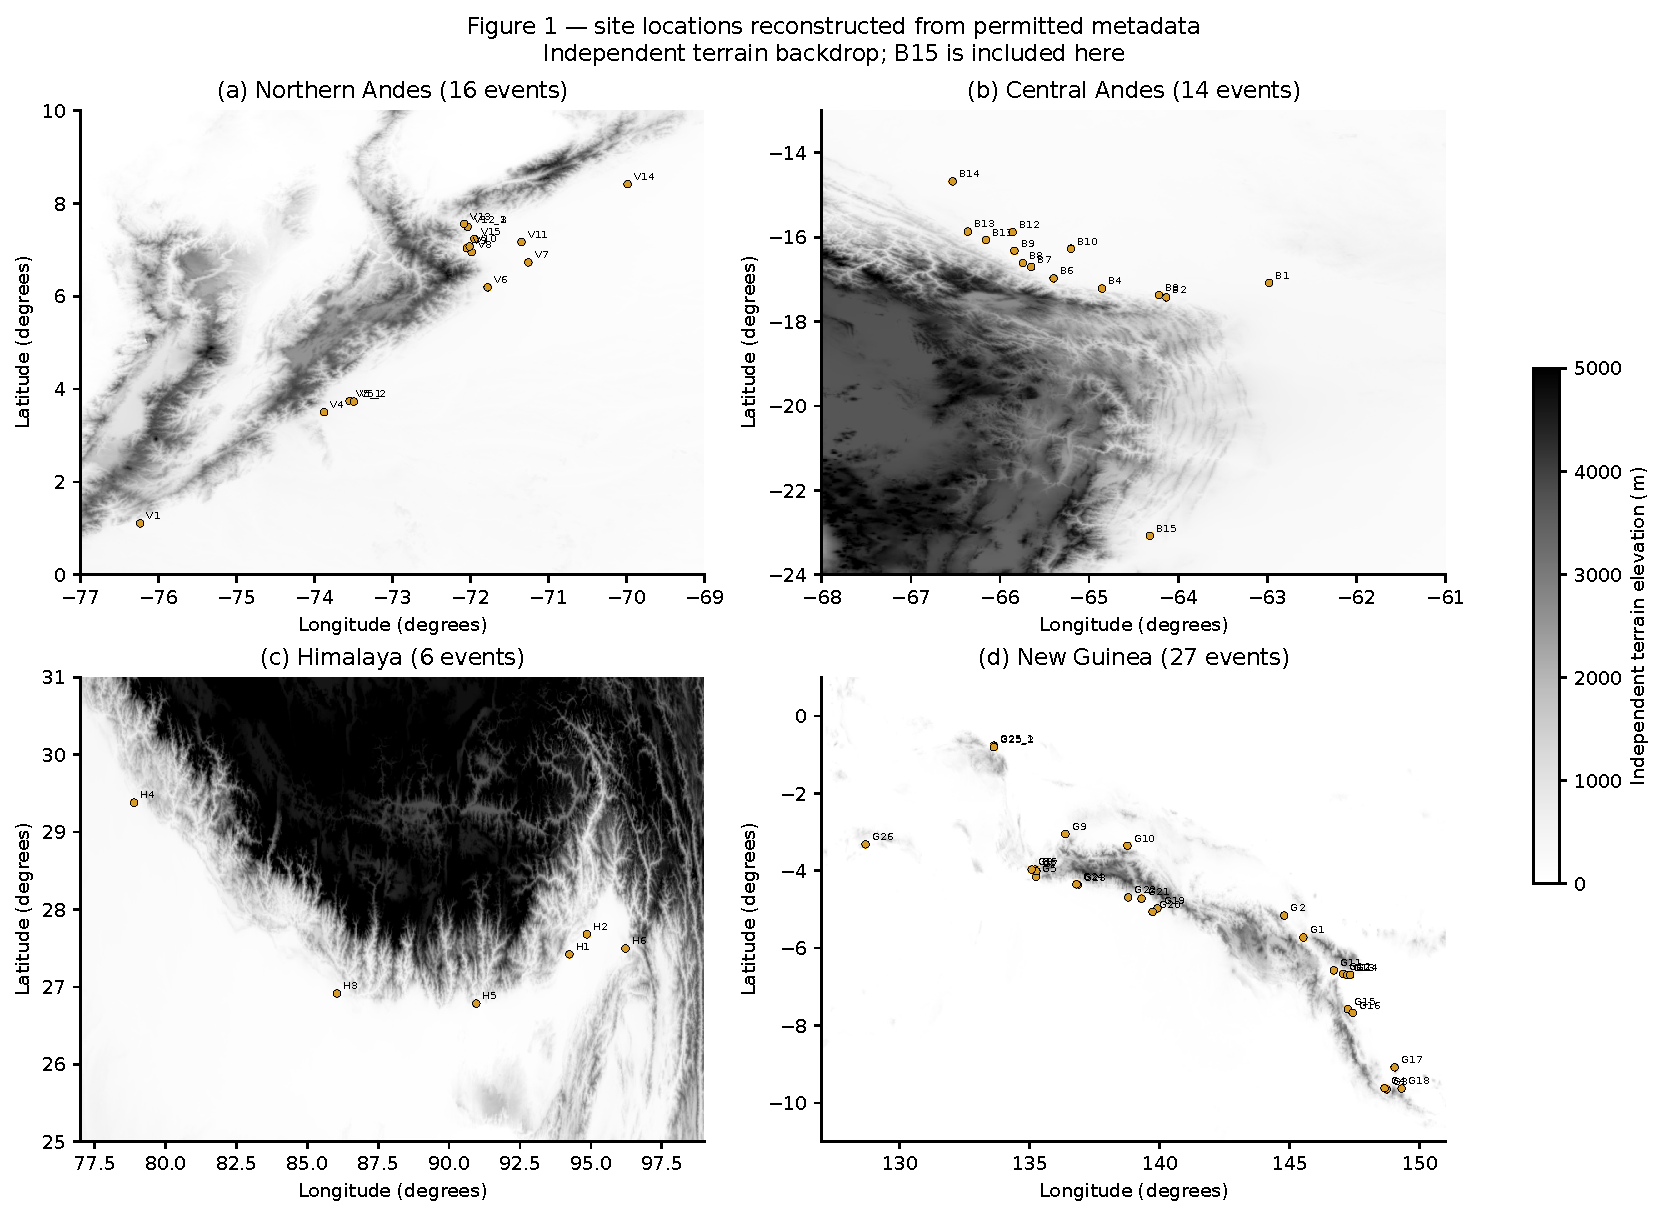
\includegraphics[width=\textwidth]{fig1.pdf}
\caption{Independent reconstruction corresponding to manuscript Fig.~1a--d.
Points are the permitted site metadata processed by the C++ catalog command.
Shading is independently resampled global Terrain Tiles elevation in meters;
it is not the paper's image or a measurement of local channel slope. Site
distribution is reproduced; cartographic styling and terrain resolution differ.
SRTM and GMTED2010 data are courtesy of USGS; ETOPO1 data are from NOAA/NCEI.}
\label{fig:locations}\end{figure}
\begin{figure}[p]\centering
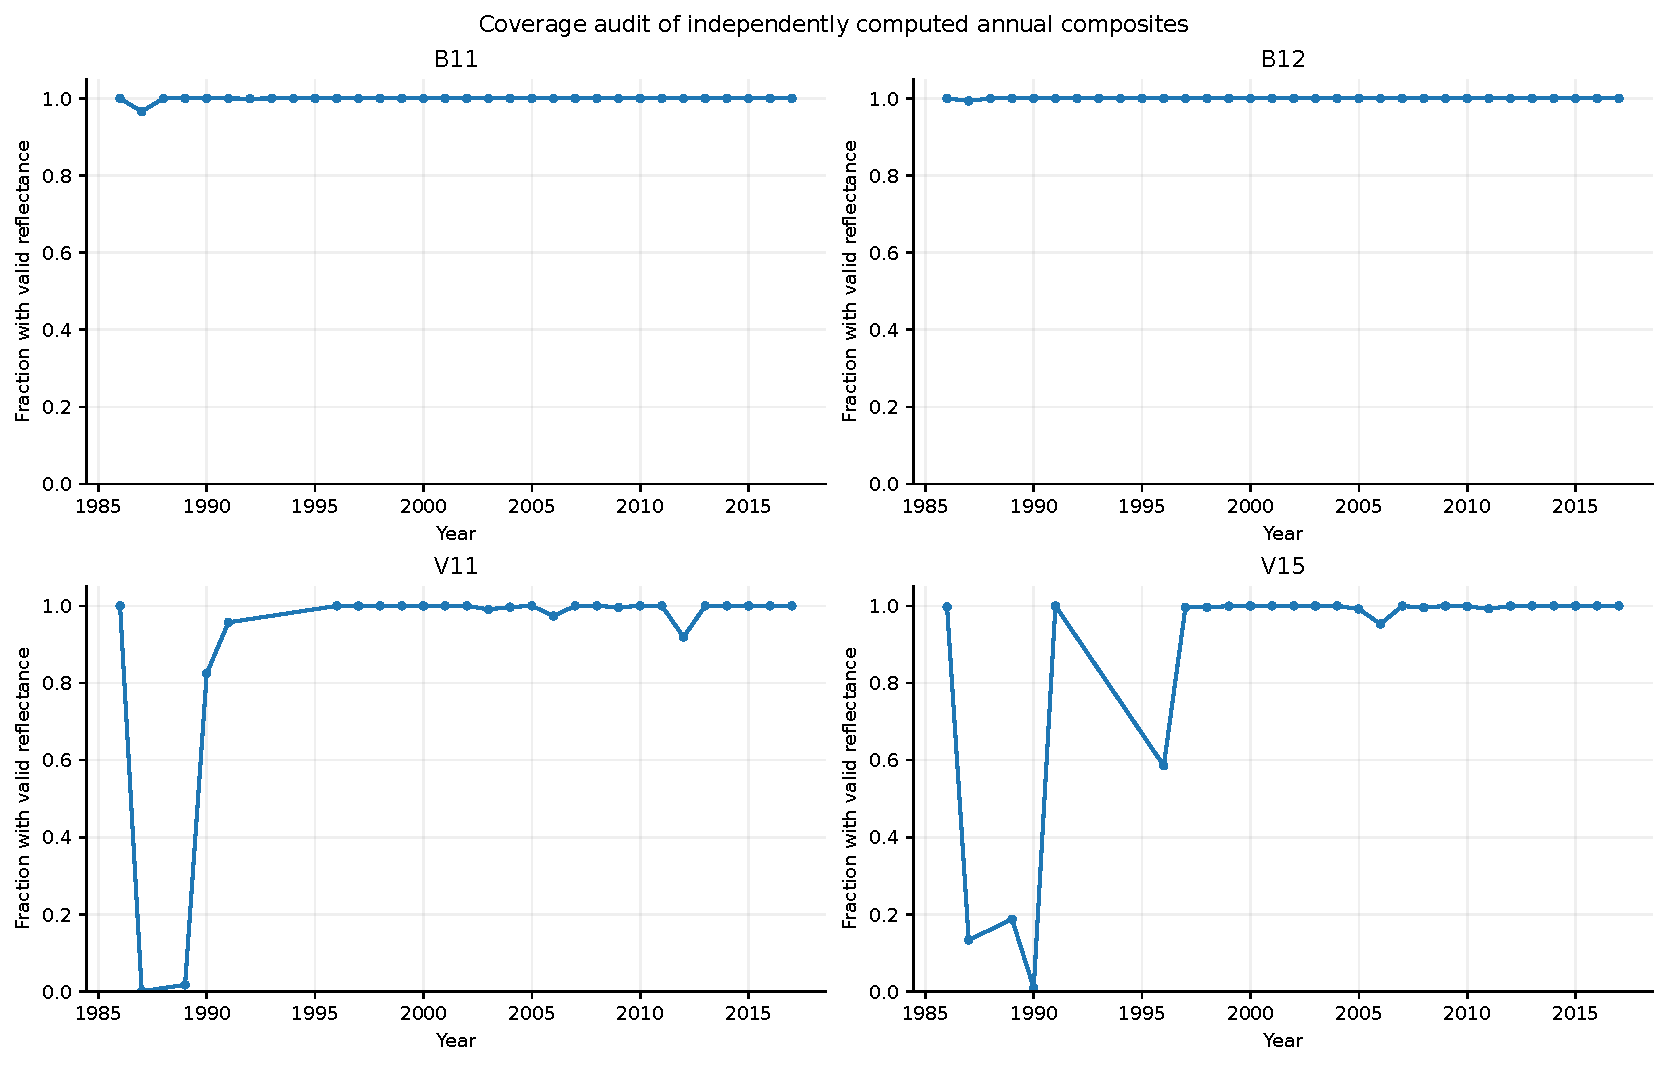
\includegraphics[width=.95\textwidth]{coverage.pdf}
\caption{Coverage of the independently calculated 30-m annual composites in
the four approximately 20-km domains. Gaps between years are shown by connecting
lines for readability, not temporal interpolation. Low coverage prevents an
absence of detections from establishing an absence of avulsion activity.}
\label{fig:coverage}\end{figure}

\subsection{The Sarare observation and its limits}
The V11 sequence shows a southern meandering course in 1986 and a northern
course with adjoining exposed surfaces in the 1990s. Parts of the northern
course are already visible in the partly cloudy 1991 composite; a complete
course is clear by 1996. The available sequence does not resolve initiation
or completion. The broad disturbed corridor also intersects the eastern
domain boundary. I therefore retain a \emph{partial} 1996--1998 footprint,
with a separate 1986 parent observation. Its vertices, inspection record,
and limitations are in \artifact{config/annotations/V11/}.

\begin{center}\small\begin{tabular}{lrrr}\toprule Signature & Parent area (km$^2$) & Partial event area (km$^2$) & Area ratio\\\midrule
B & 0.3717 & 2.7450 & 7.3850 \\
W & 2.2014 & 22.8141 & 10.3635 \\
\bottomrule\end{tabular}\end{center}
The brightness signature selects the smaller event footprint. Its area ratio
is approximately 7.38, whereas the paper reports $S_R=16.0$ for V11 in its
discussion of Fig.~5 and labels Fig.~5e with $S_R=14.9$ \cite{valenza}.
Numerically, the diagnostic is about 46.2\% and 49.6\% of these two reference
values, respectively. The publication's discrepancy is not resolved here.
These are not commensurate event estimates:
our image domain truncates the event, the windows have unequal duration,
the masks are approximate, and the spectral processing differs. No recovery
of the published $S_R$ is claimed. The wetness signature yields a much larger
partial disturbance area, demonstrating sensitivity that a single selected
number would conceal.

The V15 imagery shows a braided belt, but this attempt does not uniquely
separate one avulsion from ordinary braid migration. A V15 event mask is
therefore absent. The near-site context is independently generated, while
the corresponding fingerprint panel remains unreproduced. A straight-line
connection between V11 and V15 would not measure their along-channel
separation; only their positions are shown in the overview attempt.

\subsection{B12, B11, and the statistical panels}
At B12 the independently acquired annual composites show changes in channel
occupation. The larger domain follows the observed channel northeast and
retains the years used by Supplementary Fig.~1. The partial central-reach
footprint uses an independently drawn polygon and the 2010--2017 observation
window; its parent is a truncated old-channel segment observed in 1995.
The northeastern polygon boundary crosses the continuing channel, so its
area cannot represent the complete event. This supplies partial Fig.~2a,b
and four annual counterparts in Fig.~2c. Exact spatial agreement with
the published central splay crop cannot be established from a site coordinate
alone. At B11, narrow channels and uncertain event attribution prevent a
defensible complete fingerprint. Candidate spectral detections are preserved
as diagnostics, but they are not substitutes for avulsion masks.

\begin{center}\small\begin{tabular}{lrrr}\toprule Signature & Parent area (km$^2$) & Partial event area (km$^2$) & Area ratio\\\midrule
B & 0.6426 & 15.0012 & 23.3445 \\
W & 3.7080 & 17.6508 & 4.7602 \\
\bottomrule\end{tabular}\end{center}
The B12 table reports the partial central reach only. Brightness selects the
smaller avulsion area even though its ratio is larger than the wetness ratio.
This illustrates why the stated selection rule must operate on avulsion area,
not on the desired value of $S_R$. Neither ratio is used in the statistical
figures or compared with an author measurement table.

Post hoc inspection of manuscript Figs.~2 and 5 was restricted to assessing
agreement after these masks and windows were fixed. It exposes a material
B12 mismatch: the publication displays the parent above the disturbed
avulsion reach, whereas our limited sequence identifies an older southern
course and a later northern course. The reference has no georeferenced axes,
so display orientation alone cannot establish a north/south reversal.
Orientation, a different relocation phase, or incorrect event attribution
could explain the unmatched layouts. The present data do not resolve it.
Thus the B12 panels are partial spectral-method attempts, not a verified
reconstruction of the publication's event or spatial progression. No input
polygon was adjusted to resemble the reference.

The published Fig.~2 duration legend reaches 20 years; our selected window
contains eight. The reference's annual counterparts are 2007, 2010, 2013,
and 2017, whereas the previously declared attempt years are 2011, 2013, 2015,
and 2017. Those attempt years remain unchanged. The reference validation dates
are 30 November 2007, 2 November 2010, 19 August 2013, and 30 August 2017;
they are comparison information only. Their commercial images were not
independently acquired. The V11 reference also includes extensive southern
disturbance omitted by our northern polygon. These comparisons support the
partial status rather than numerical validation. The assessment is archived
in \artifact{docs/published-comparison.md}.

\subsection{Sensitivity to the analysis domain}
The nested B12 domains permit a numerical comparison over identical physical
pixels. The C++ comparison maps their aligned 30-m grids, retains pixels valid
in both composites, and reports foreground intersection-over-union and total
pixel agreement for each spectral signature. Mean absolute RGB difference is
in reflectance units. Zero difference would establish agreement of the visible
bands only; the other spectral bands and transforms would still need checking.
Nonzero differences can reflect sensor selection, scene composition, or
reprojection. This is a combined domain-sensitivity assessment, not an isolated
threshold experiment.

\begin{center}\small\IfFileExists{domain_table.tex}{\begin{tabular}{lrrrr}\toprule Year & Signature & Intersection/union & Pixel agreement & Mean RGB difference\\\midrule
1995 & B & 0.569 & 0.993 & 9.862e-05 \\
1995 & W & 0.242 & 0.906 & 9.862e-05 \\
2010 & B & 0.517 & 0.985 & 3.853e-05 \\
2010 & W & 0.175 & 0.946 & 3.853e-05 \\
2011 & B & 0.510 & 0.991 & 6.038e-05 \\
2011 & W & 0.121 & 0.861 & 6.038e-05 \\
2012 & B & 0.381 & 0.994 & 4.921e-05 \\
2012 & W & 0.247 & 0.846 & 4.921e-05 \\
2013 & B & 0.273 & 0.981 & 0.002775 \\
2013 & W & 0.163 & 0.947 & 0.002775 \\
2014 & B & 0.610 & 0.992 & 4.84e-05 \\
2014 & W & 0.275 & 0.960 & 4.84e-05 \\
2015 & B & 0.429 & 0.990 & 5.193e-05 \\
2015 & W & 0.282 & 0.965 & 5.193e-05 \\
2016 & B & 0.390 & 0.978 & 4.298e-05 \\
2016 & W & 0.288 & 0.968 & 4.298e-05 \\
2017 & B & 0.152 & 0.977 & 0.003954 \\
2017 & W & 0.214 & 0.875 & 0.003954 \\
\bottomrule\end{tabular}}{}\end{center}
Overall agreement can be dominated by background pixels, so it is reported
alongside foreground overlap. This comparison is an internal sensitivity
assessment, not agreement with a published mask. It demonstrates why a
geographic site coordinate alone does not fully specify a fingerprint.
The command is
\texttt{build/avulsion compare-domains data/derived/B12
data/derived/B12\_wide data/results/domain\_sensitivity.csv}.

The independently acquired Landsat data have 30-m pixels, each representing
900~m$^2$. A three-pixel boundary uncertainty is already 90~m. The commercial
WorldView validation images in manuscript Fig.~2c and Supplementary Fig.~2c
were not independently acquired. Consequently, this project cannot calculate
pixel precision, recall, intersection-over-union, or progradation-front error
against those observations. No published image is digitized to manufacture
such scores.

Figures~3a,b, 4, and S3a,b remain unreproduced. The arithmetic for their
quantities is implemented and tested, but no complete independent event and
channel-geometry record supplies their plots. Empty CSVs and explicit absence
notices are preserved. A 63-point regression, median morphology contrast,
or significance claim would require measurements that this attempt did not
make. There is no numerical confirmation or refutation of the paper's central
downstream relationship.

\clearpage
\section{Figure attempts}
These pages identify every main and supplementary figure. A generated image
can constitute a partial attempt while failing to reproduce the intended
scientific quantity. In particular, a missing-data notice is never counted
as a reproduced panel. The detailed ledger following these pages gives
panel-level quantities, parameters, exact commands, and limitations.

\begin{figure}[p]\centering
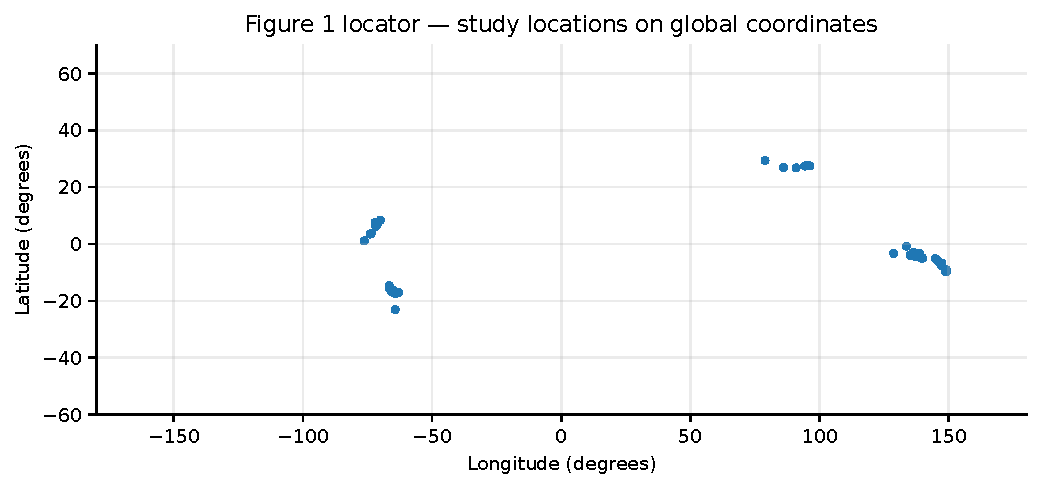
\includegraphics[width=.94\textwidth]{fig1_locator.pdf}
\caption{Manuscript Fig.~1 locator attempt. The global coordinates are generated
from the permitted metadata; continental outlines and the original inset
design are absent. This is a partial geographic context plot.}
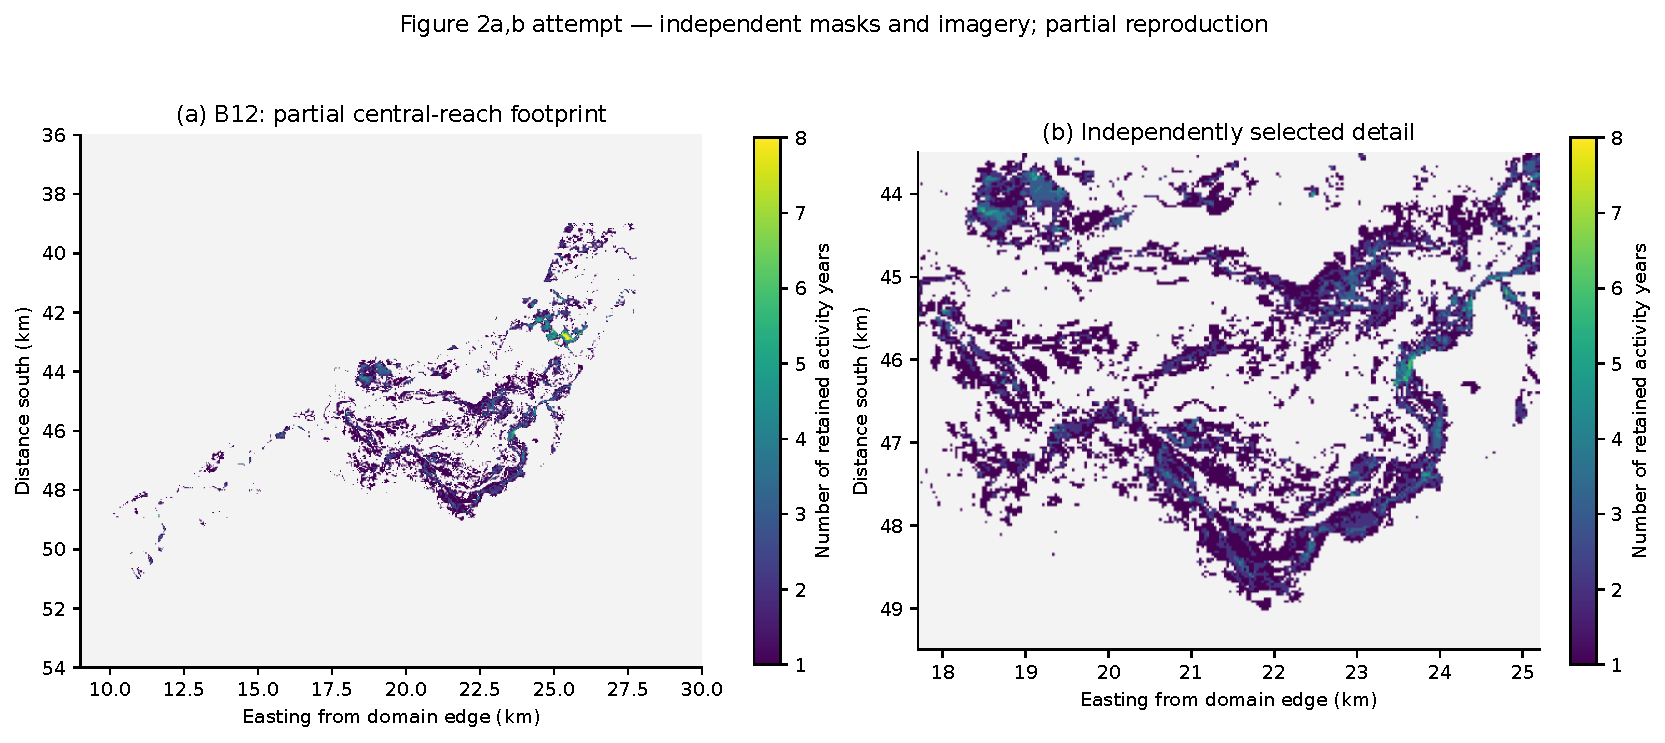
\includegraphics[width=\textwidth]{fig2ab.pdf}
\caption{Manuscript Fig.~2a,b attempt. A valid generated footprint, if available,
uses only the independent imagery and annotations. An absence notice identifies
a missing scientific result; it must not be interpreted as a zero-area event.}
\end{figure}
\begin{figure}[p]\centering
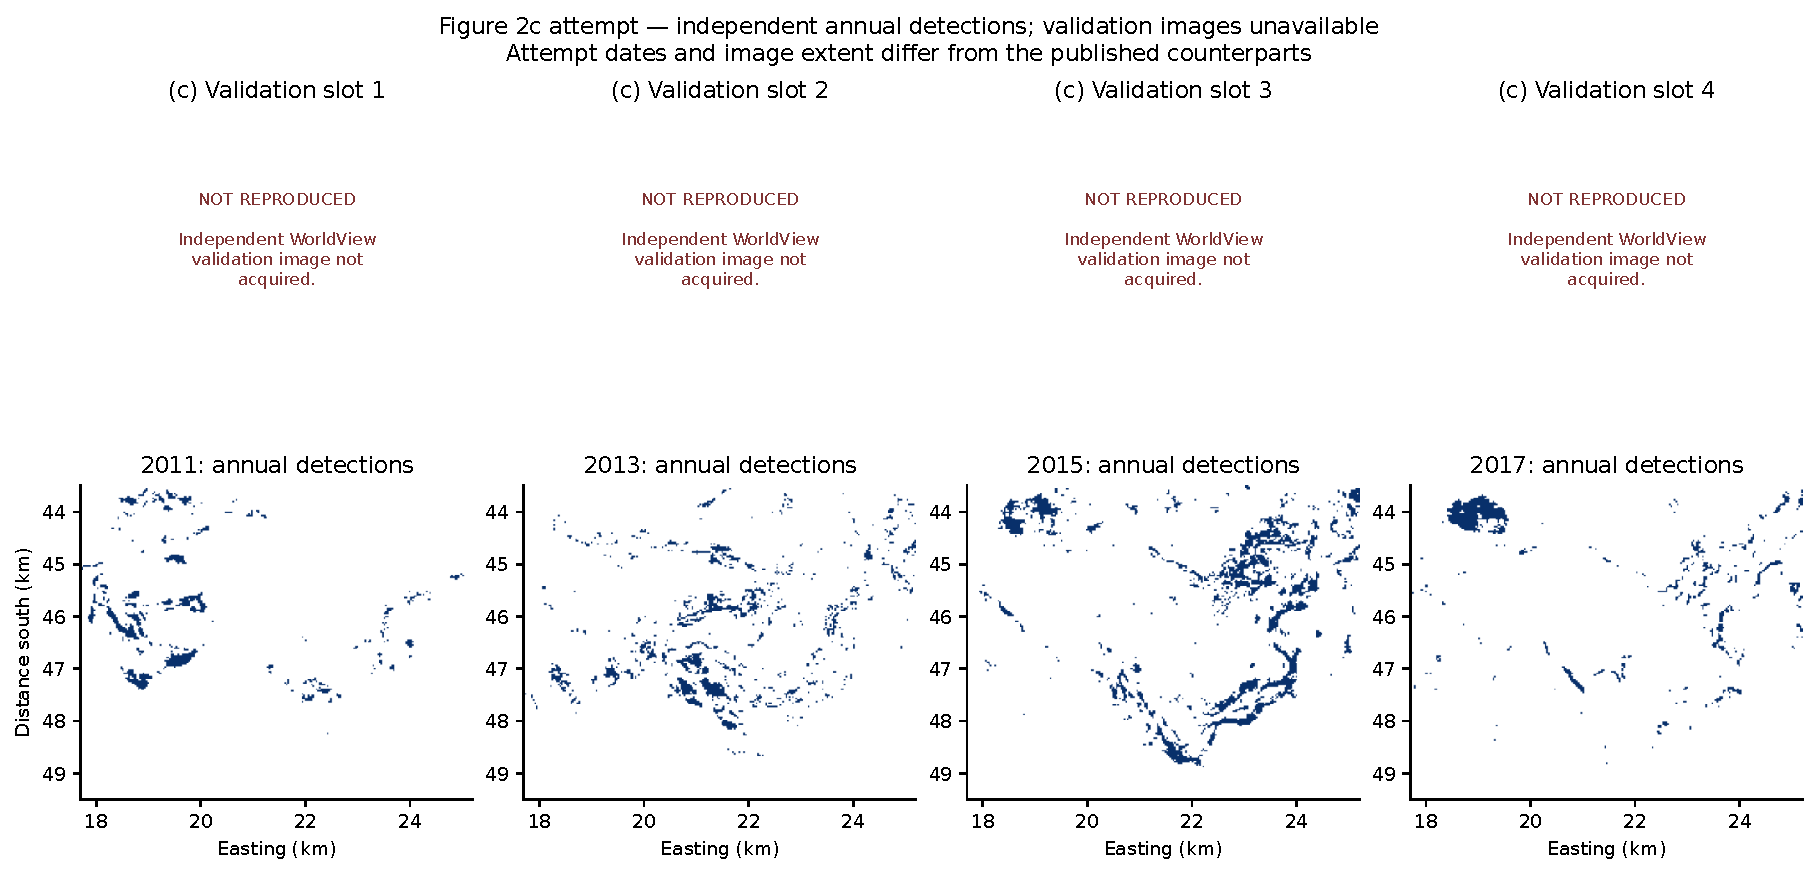
\includegraphics[width=\textwidth]{fig2c.pdf}
\caption{Manuscript Fig.~2c attempt, with four upper validation slots and four
lower annual-detection slots. Independently acquired WorldView observations
are unavailable. Attempt years 2011, 2013, 2015, and 2017 are explicit choices,
not the published annual counterparts 2007, 2010, 2013, and 2017. The latter
were identified only during post hoc comparison and did not change the inputs.}
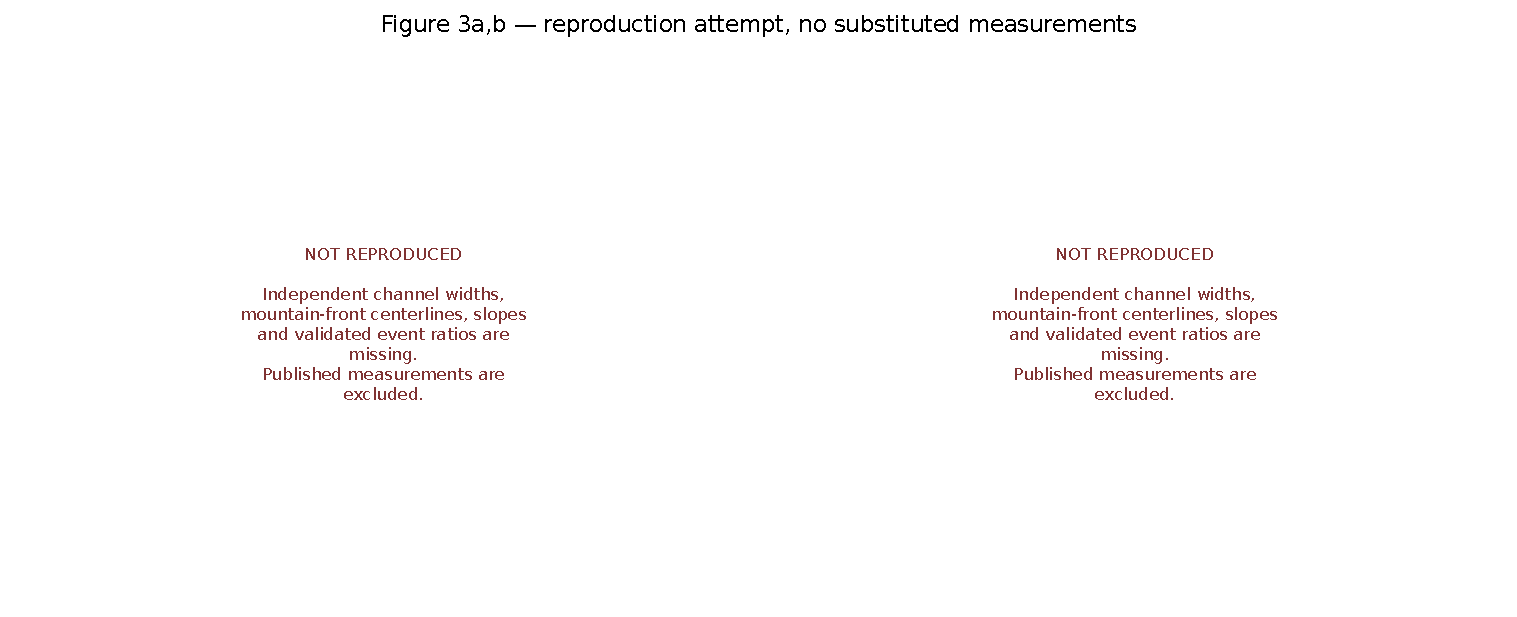
\includegraphics[width=\textwidth]{fig3.pdf}
\caption{Manuscript Fig.~3a,b accounting panels. Missing independent channel
geometry and complete event ratios prevent either statistical comparison.
No published point coordinates or synthetic observations are plotted.}
\end{figure}
\begin{figure}[p]\centering
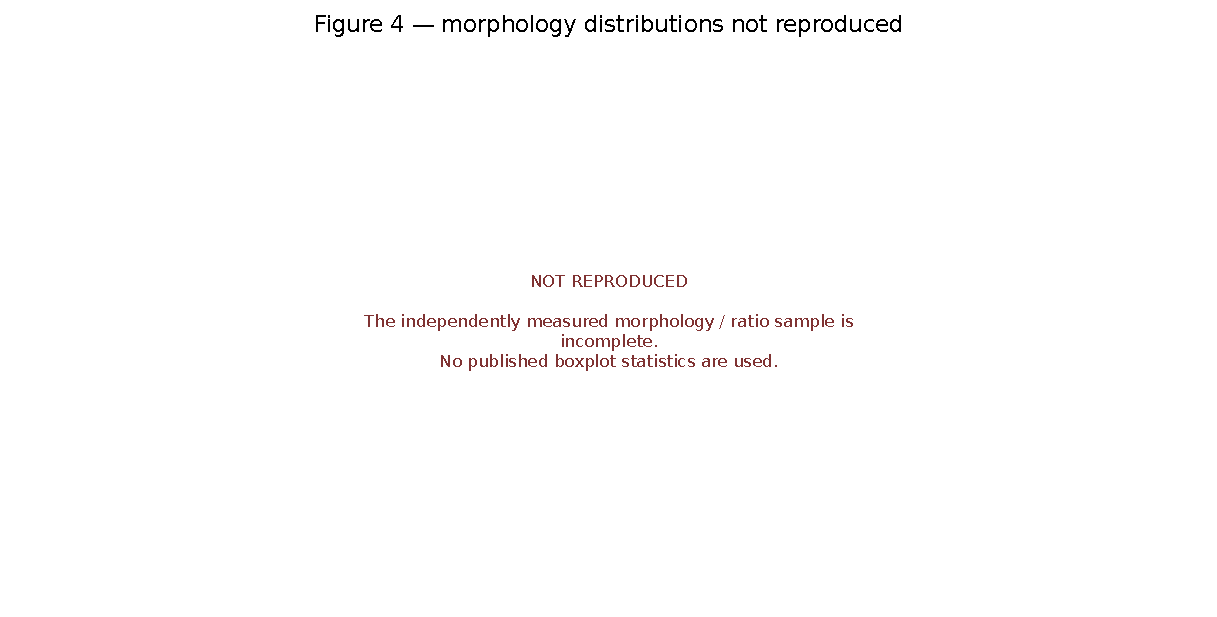
\includegraphics[width=.94\textwidth]{fig4.pdf}
\caption{Manuscript Fig.~4 accounting panel. The independently measured
morphology--style-ratio sample is empty; no boxplot can be reproduced.}
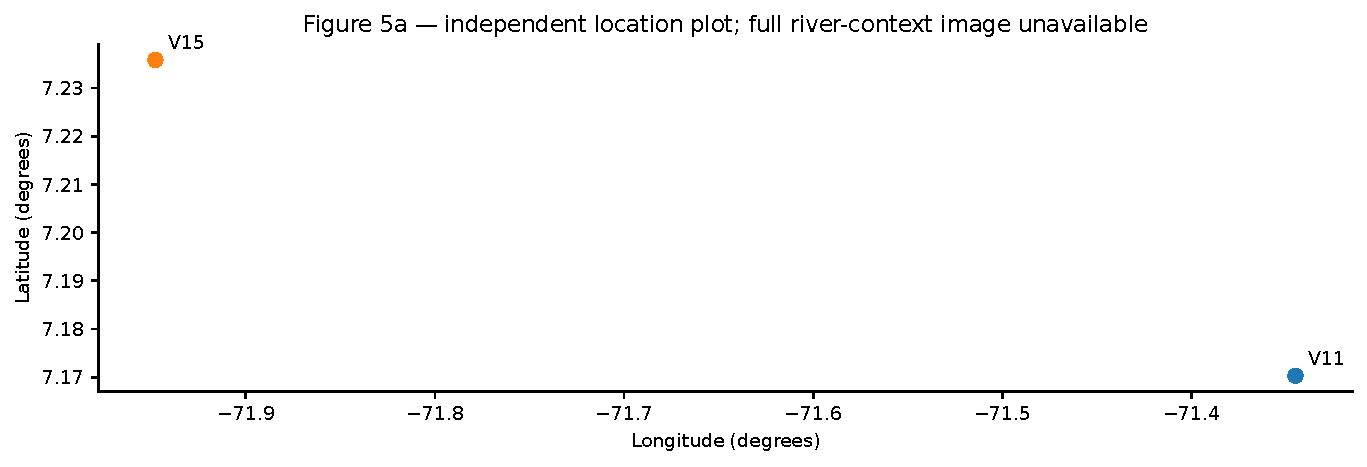
\includegraphics[width=.94\textwidth]{fig5a.pdf}
\caption{Manuscript Fig.~5a partial attempt. The independently plotted site
positions do not replace the paper's river-context mosaic or measure
along-channel distance.}
\end{figure}
\begin{figure}[p]\centering
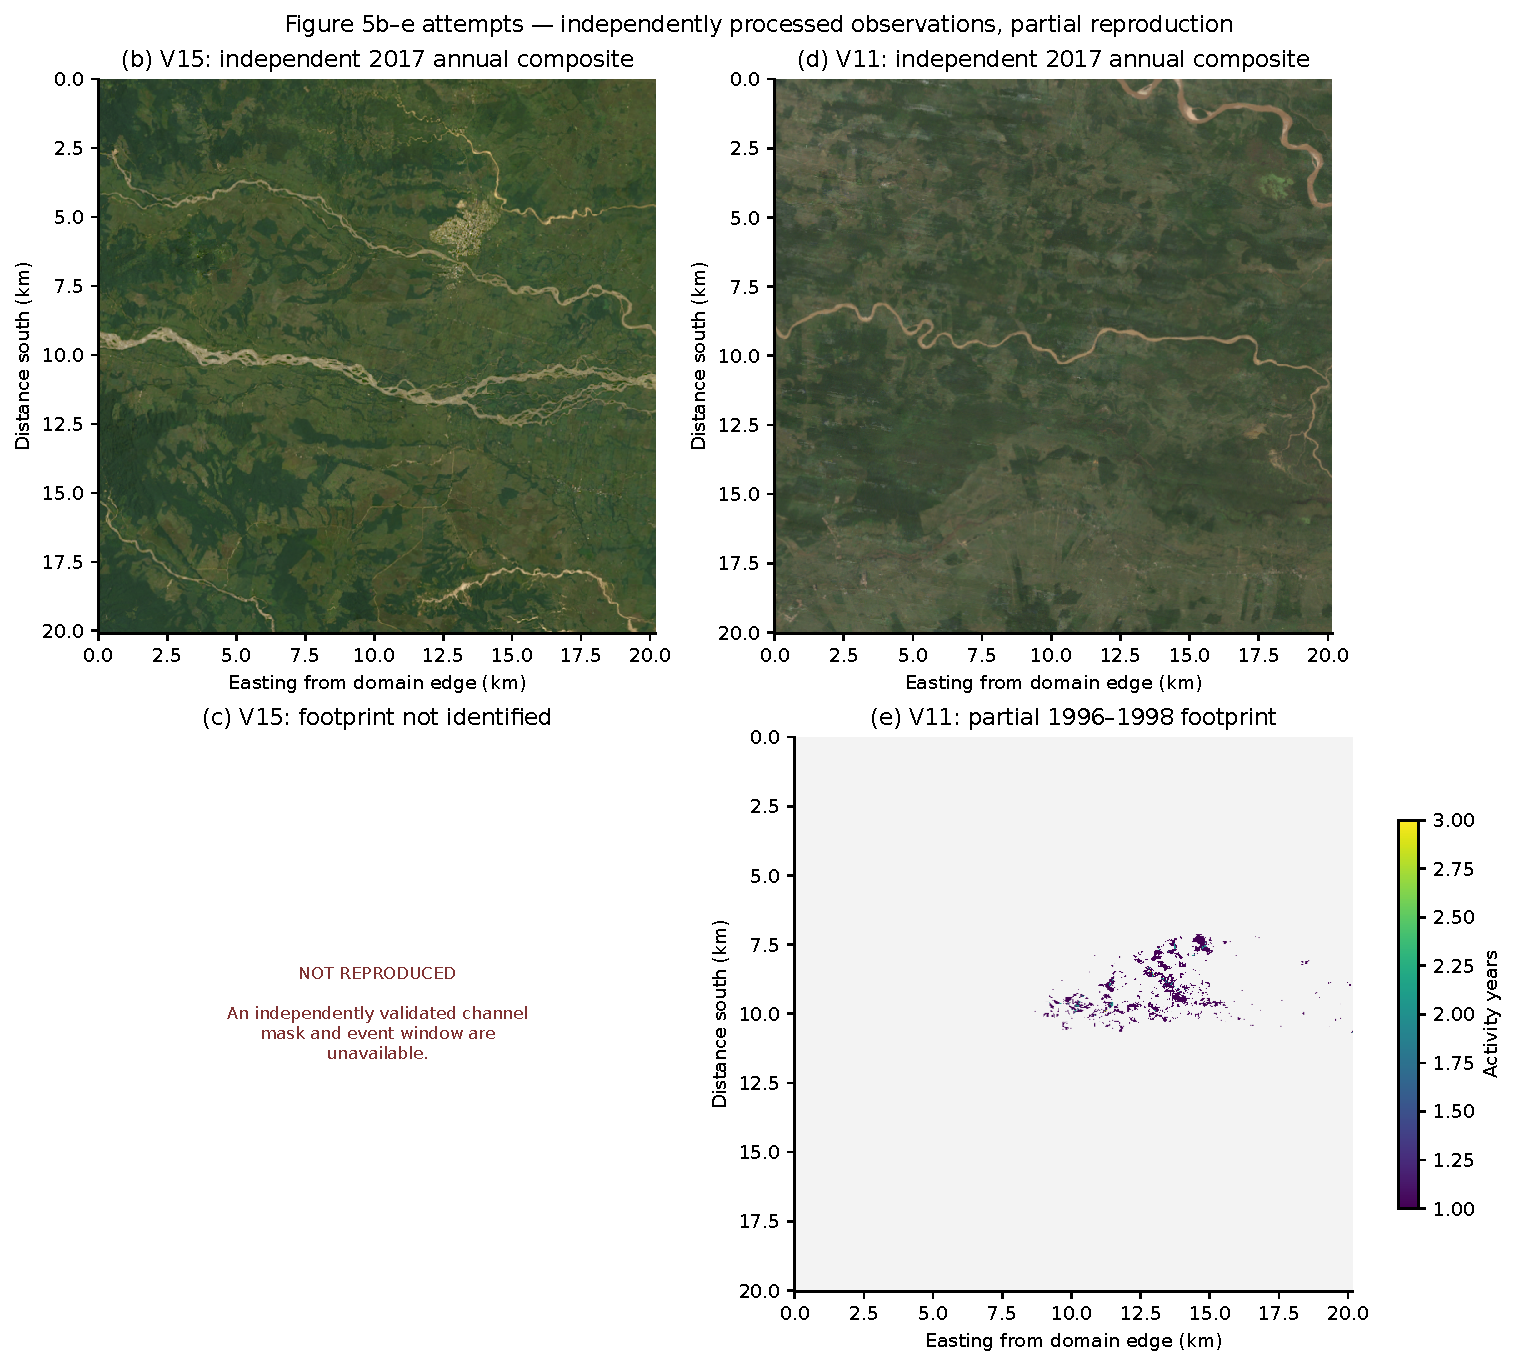
\includegraphics[width=.94\textwidth]{fig5bcde.pdf}
\caption{Manuscript Fig.~5b--e attempts. Top: independent 2017 annual RGB
composites, displayed with the same fixed stretch. These differ from the
paper's 2019 Google Earth context images. Bottom left: V15 event not identified.
Bottom right: V11's partial 1996--1998 duration fingerprint, using the selected
brightness signature and an independently drawn polygon. The event crosses
the eastern domain edge; this is not a complete event or a validated style
ratio. Colors count retained years of spectral detection.}
\end{figure}
\begin{figure}[p]\centering
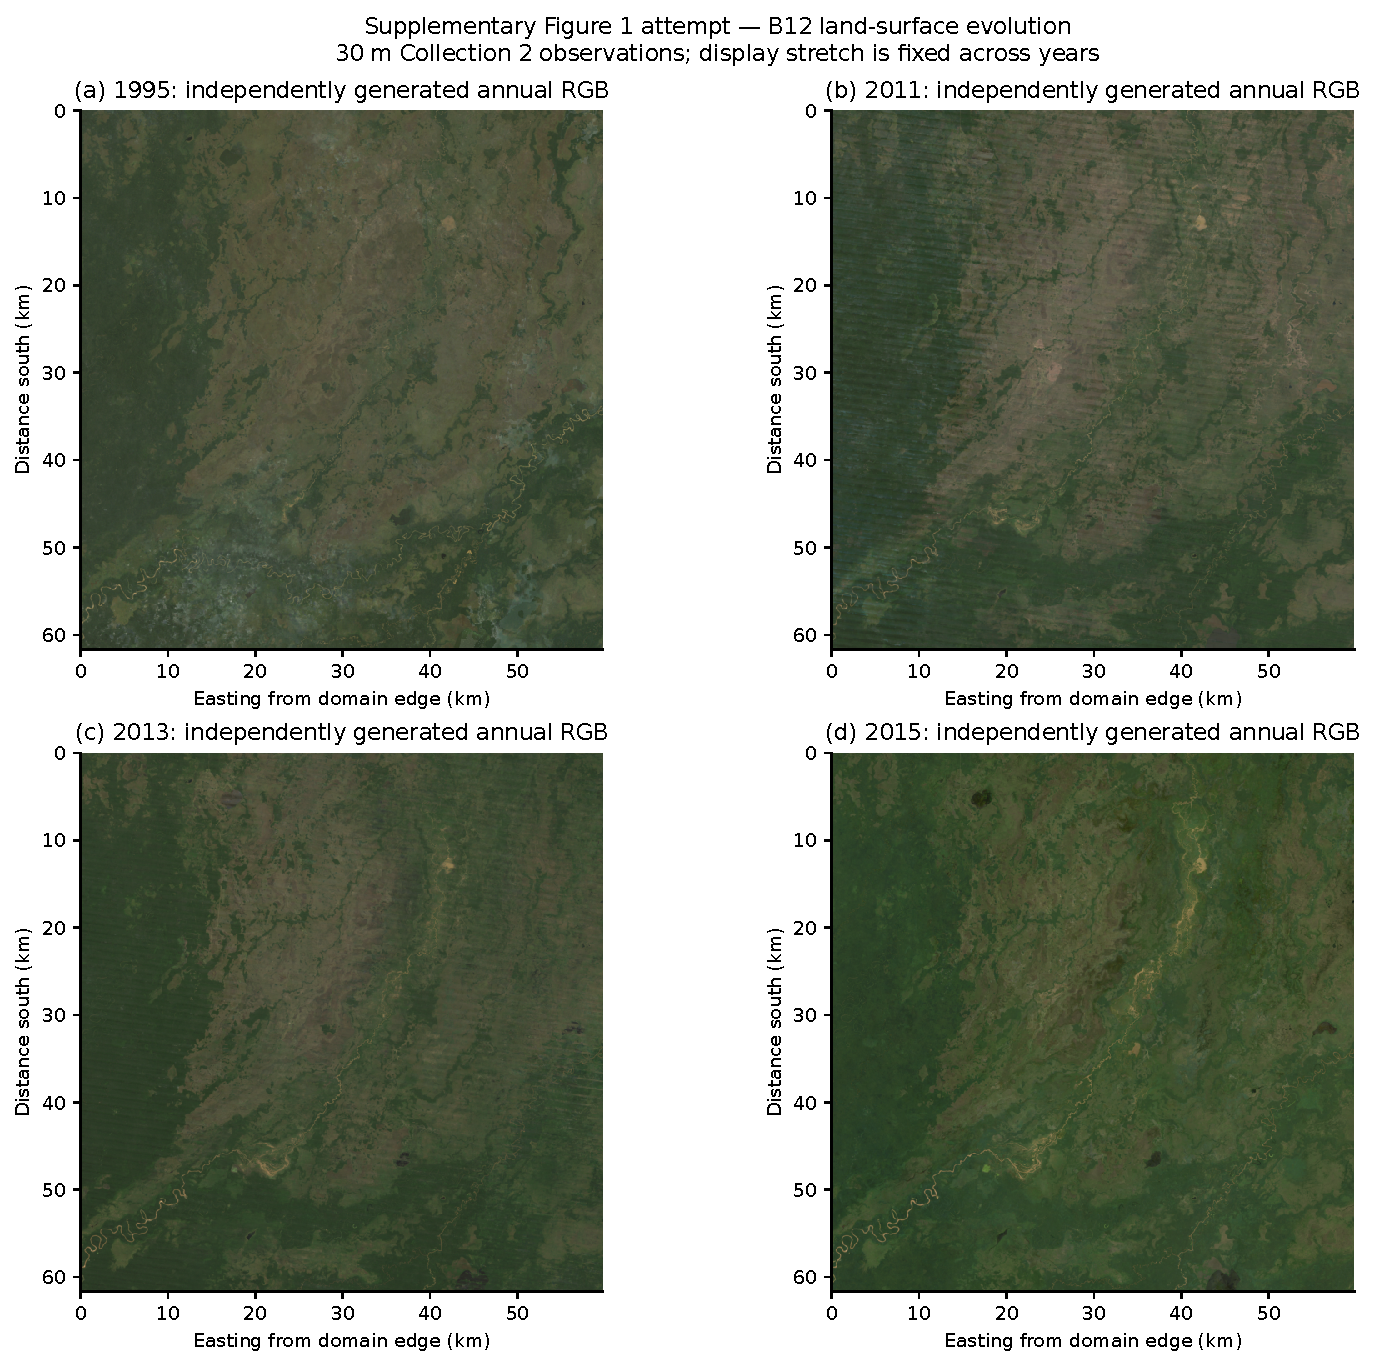
\includegraphics[width=.96\textwidth]{supp1.pdf}
\caption{Supplementary Fig.~1a--d attempts: independent B12 annual RGB
composites for 1995, 2011, 2013, and 2015 on the larger 30-m domain. The
stretch divides reflectance by 0.35 and applies exponent $1/1.6$; missing
pixels are gray. These are partial observations with independently chosen
extent, not copies of the publication's panels.}
\end{figure}
\begin{figure}[p]\centering

\includegraphics[width=\textwidth]{supp2.pdf}
\caption{Supplementary Fig.~2a--c attempts. A complete B11 fingerprint and
the independent WorldView validation observation of 8 July 2016 remain
unavailable. The missing-result notices are not reproduced scientific panels.}
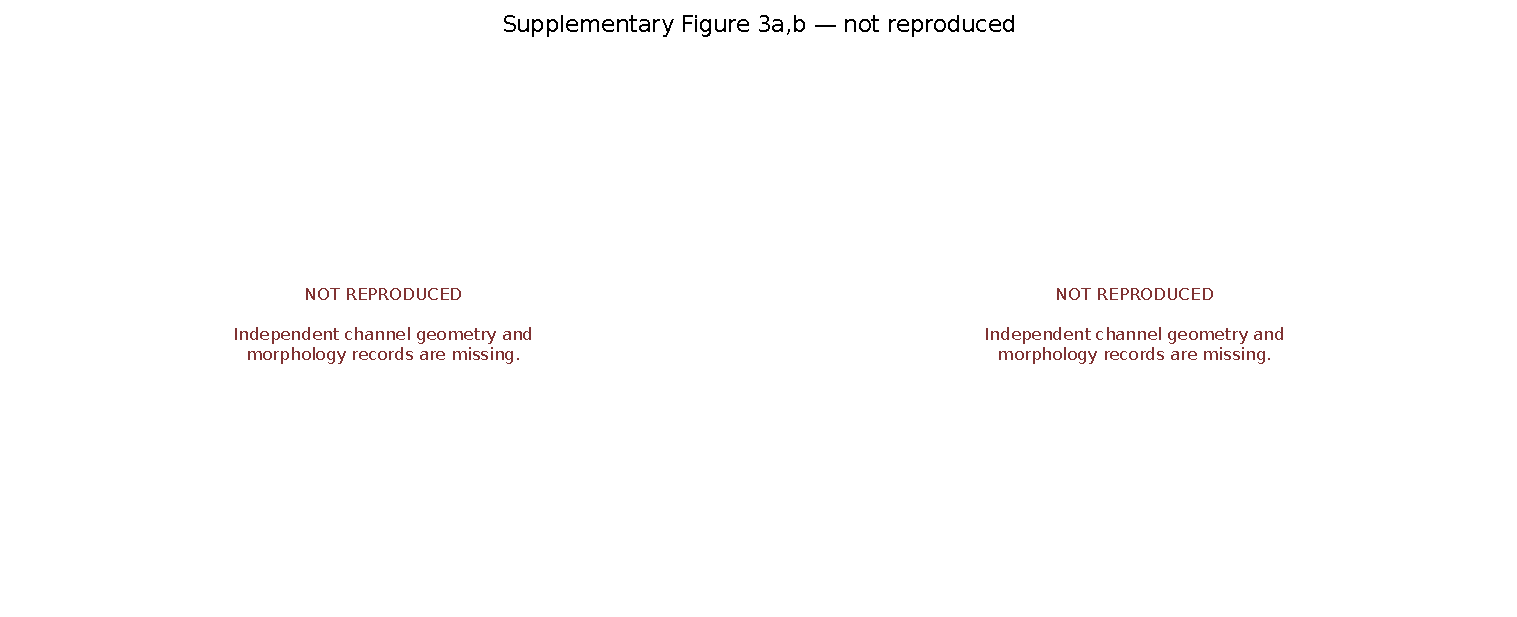
\includegraphics[width=\textwidth]{supp3.pdf}
\caption{Supplementary Fig.~3a,b accounting panels. Independent slope,
normalized distance, and morphology measurements remain incomplete.}
\end{figure}
\begin{figure}[p]\centering
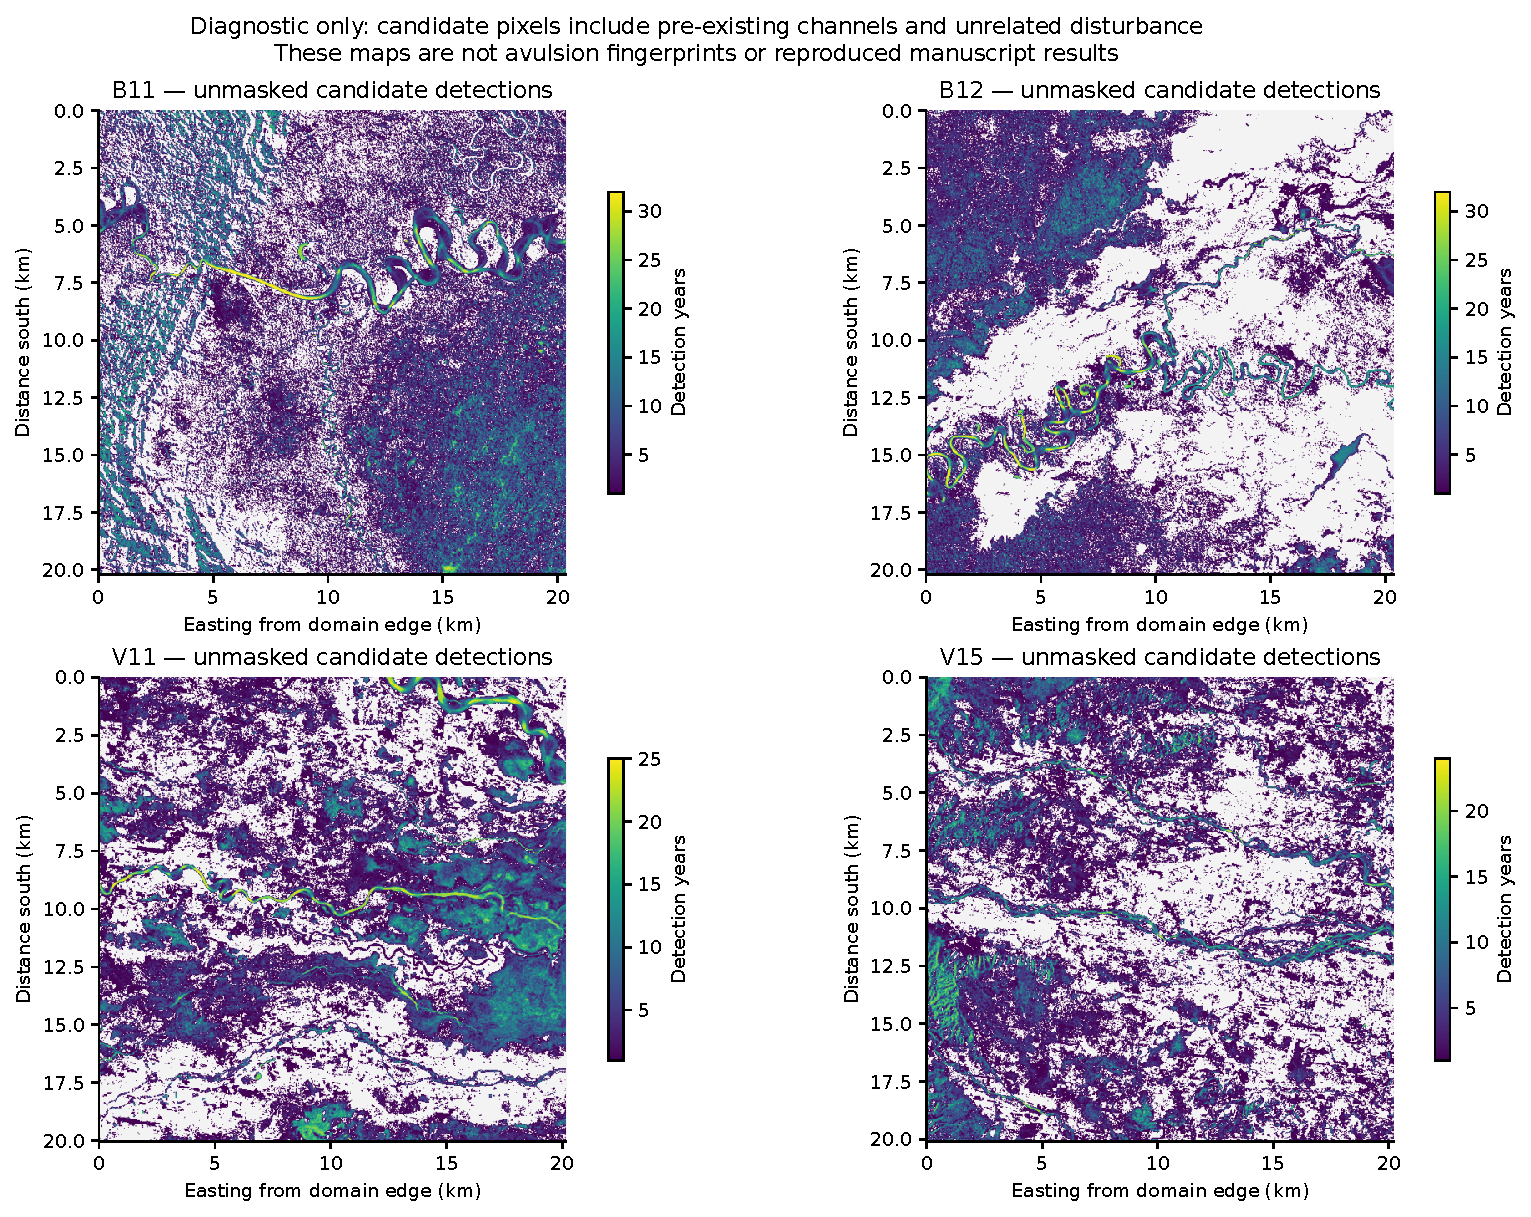
\includegraphics[width=\textwidth]{candidate_diagnostics.pdf}
\caption{Additional diagnostic, not a manuscript reproduction. Unmasked
wetness-signature detection-year counts include pre-existing rivers, clouds
that escape the alternate screen, and unrelated disturbance. The accumulation
uses all available years and is not an avulsion event footprint.}
\end{figure}

\clearpage
\section{Panel-by-panel record}
``Independently reproduced'' is restricted here to the geographic site
distribution in Fig.~1a--d, generated by this implementation from permitted
location metadata and independent terrain. It does not denote a reproduced
model prediction or identical cartography. ``Partially reproduced'' denotes
generated observations with stated departures or missing components.
``Not reproduced'' denotes absence of the panel's scientific quantity.
The machine-readable version is \artifact{data/results/panel_record.csv}.
Commands are relative to the repository root; the acquisition and build
prerequisites are given below. A missing-annotation command records the
unsatisfied prerequisite and is not run by the successful default procedure.
\begingroup\small\subsubsection*{Panel 1a --- independently reproduced}
Site distribution: Northern Andes (16). Main Fig. 1 caption; permitted site coordinates.

\textit{Parameters:} 63 coordinates overall; independent zoom-7 terrain resampled to 600 x 800; B15 included.

\textit{Data:} \texttt{build/\allowbreak{}avulsion catalog config/\allowbreak{}sites.csv data/\allowbreak{}results; .runtime/\allowbreak{}py311/\allowbreak{}bin/\allowbreak{}python scripts/\allowbreak{}terrain.py}.

\textit{Plot:} \texttt{.runtime/\allowbreak{}py311/\allowbreak{}bin/\allowbreak{}python scripts/\allowbreak{}plot.py --figure fig1}.

Reproduces the geographic site distribution, not pixel-identical cartography. Background source, map bounds and label placement differ. This is an observational map, not a model result.

\subsubsection*{Panel 1b --- independently reproduced}
Site distribution: Central Andes (14). Main Fig. 1 caption; permitted site coordinates.

\textit{Parameters:} 63 coordinates overall; independent zoom-7 terrain resampled to 600 x 800; B15 included.

\textit{Data:} \texttt{build/\allowbreak{}avulsion catalog config/\allowbreak{}sites.csv data/\allowbreak{}results; .runtime/\allowbreak{}py311/\allowbreak{}bin/\allowbreak{}python scripts/\allowbreak{}terrain.py}.

\textit{Plot:} \texttt{.runtime/\allowbreak{}py311/\allowbreak{}bin/\allowbreak{}python scripts/\allowbreak{}plot.py --figure fig1}.

Reproduces the geographic site distribution, not pixel-identical cartography. Background source, map bounds and label placement differ. This is an observational map, not a model result.

\subsubsection*{Panel 1c --- independently reproduced}
Site distribution: Himalaya (6). Main Fig. 1 caption; permitted site coordinates.

\textit{Parameters:} 63 coordinates overall; independent zoom-7 terrain resampled to 600 x 800; B15 included.

\textit{Data:} \texttt{build/\allowbreak{}avulsion catalog config/\allowbreak{}sites.csv data/\allowbreak{}results; .runtime/\allowbreak{}py311/\allowbreak{}bin/\allowbreak{}python scripts/\allowbreak{}terrain.py}.

\textit{Plot:} \texttt{.runtime/\allowbreak{}py311/\allowbreak{}bin/\allowbreak{}python scripts/\allowbreak{}plot.py --figure fig1}.

Reproduces the geographic site distribution, not pixel-identical cartography. Background source, map bounds and label placement differ. This is an observational map, not a model result.

\subsubsection*{Panel 1d --- independently reproduced}
Site distribution: New Guinea (27). Main Fig. 1 caption; permitted site coordinates.

\textit{Parameters:} 63 coordinates overall; independent zoom-7 terrain resampled to 600 x 800; B15 included.

\textit{Data:} \texttt{build/\allowbreak{}avulsion catalog config/\allowbreak{}sites.csv data/\allowbreak{}results; .runtime/\allowbreak{}py311/\allowbreak{}bin/\allowbreak{}python scripts/\allowbreak{}terrain.py}.

\textit{Plot:} \texttt{.runtime/\allowbreak{}py311/\allowbreak{}bin/\allowbreak{}python scripts/\allowbreak{}plot.py --figure fig1}.

Reproduces the geographic site distribution, not pixel-identical cartography. Background source, map bounds and label placement differ. This is an observational map, not a model result.

\subsubsection*{Panel 1 locator --- partially reproduced}
Global study-region locations. Main Fig. 1.

\textit{Parameters:} Same coordinates; rectangular longitude/latitude axes.

\textit{Data:} \texttt{build/\allowbreak{}avulsion catalog config/\allowbreak{}sites.csv data/\allowbreak{}results}.

\textit{Plot:} \texttt{.runtime/\allowbreak{}py311/\allowbreak{}bin/\allowbreak{}python scripts/\allowbreak{}plot.py --figure fig1}.

Global positions generated independently; continental outline and original inset design absent.

\subsubsection*{Panel 2a --- partially reproduced}
Cumulative B12 disturbance footprint. Main Fig. 2 caption; Methods fingerprinting; Supplementary Table 2.

\textit{Parameters:} 30 m; B90/G50 and W75/G50; independent rectangular domain and manual polygon if available.

\textit{Data:} \texttt{build/\allowbreak{}avulsion analyze data/\allowbreak{}raw/\allowbreak{}B12\_wide data/\allowbreak{}derived/\allowbreak{}B12\_wide; build/\allowbreak{}avulsion measure data/\allowbreak{}derived/\allowbreak{}B12\_wide config/\allowbreak{}annotations/\allowbreak{}B12\_wide/\allowbreak{}polygons.csv data/\allowbreak{}derived/\allowbreak{}B12\_wide/\allowbreak{}event}.

\textit{Plot:} \texttt{.runtime/\allowbreak{}py311/\allowbreak{}bin/\allowbreak{}python scripts/\allowbreak{}plot.py --figure fig2}.

Published spatial pattern and parent/new-channel relationship are not recovered. This is a partial spectral-method attempt, not a verified reconstruction of the published event. See docs/published-comparison.md.

\subsubsection*{Panel 2b --- partially reproduced}
Detail of B12 disturbance footprint. Main Fig. 2 caption; Methods fingerprinting; Supplementary Table 2.

\textit{Parameters:} 30 m; B90/G50 and W75/G50; independent rectangular domain and manual polygon if available.

\textit{Data:} \texttt{build/\allowbreak{}avulsion analyze data/\allowbreak{}raw/\allowbreak{}B12\_wide data/\allowbreak{}derived/\allowbreak{}B12\_wide; build/\allowbreak{}avulsion measure data/\allowbreak{}derived/\allowbreak{}B12\_wide config/\allowbreak{}annotations/\allowbreak{}B12\_wide/\allowbreak{}polygons.csv data/\allowbreak{}derived/\allowbreak{}B12\_wide/\allowbreak{}event}.

\textit{Plot:} \texttt{.runtime/\allowbreak{}py311/\allowbreak{}bin/\allowbreak{}python scripts/\allowbreak{}plot.py --figure fig2}.

Published spatial pattern and parent/new-channel relationship are not recovered. This is a partial spectral-method attempt, not a verified reconstruction of the published event. See docs/published-comparison.md.

\subsubsection*{Panel 2c upper 1 --- not reproduced}
High-resolution validation observation. Main Fig. 2 caption.

\textit{Parameters:} WorldView imagery; published dates recorded only for post hoc comparison.

\textit{Data:} \texttt{No data command: independently licensed validation image unavailable}.

\textit{Plot:} \texttt{.runtime/\allowbreak{}py311/\allowbreak{}bin/\allowbreak{}python scripts/\allowbreak{}plot.py --figure fig2}.

An explicit absence notice occupies this slot. No copied validation image is displayed.

\subsubsection*{Panel 2c lower 1 --- partially reproduced}
Annual B12 detection counterpart (attempt year 2011). Main Fig. 2 caption; Methods; Supplementary Table 2.

\textit{Parameters:} 30 m annual median; selected signature; four attempt years are independently declared.

\textit{Data:} \texttt{build/\allowbreak{}avulsion analyze data/\allowbreak{}raw/\allowbreak{}B12\_wide data/\allowbreak{}derived/\allowbreak{}B12\_wide; build/\allowbreak{}avulsion measure data/\allowbreak{}derived/\allowbreak{}B12\_wide config/\allowbreak{}annotations/\allowbreak{}B12\_wide/\allowbreak{}polygons.csv data/\allowbreak{}derived/\allowbreak{}B12\_wide/\allowbreak{}event}.

\textit{Plot:} \texttt{.runtime/\allowbreak{}py311/\allowbreak{}bin/\allowbreak{}python scripts/\allowbreak{}plot.py --figure fig2}.

Published annual counterparts are 2007, 2010, 2013, 2017, identified only during post hoc assessment; our declared years remain unchanged. High-resolution counterparts unavailable; no pixel agreement score can be computed.

\subsubsection*{Panel 2c upper 2 --- not reproduced}
High-resolution validation observation. Main Fig. 2 caption.

\textit{Parameters:} WorldView imagery; published dates recorded only for post hoc comparison.

\textit{Data:} \texttt{No data command: independently licensed validation image unavailable}.

\textit{Plot:} \texttt{.runtime/\allowbreak{}py311/\allowbreak{}bin/\allowbreak{}python scripts/\allowbreak{}plot.py --figure fig2}.

An explicit absence notice occupies this slot. No copied validation image is displayed.

\subsubsection*{Panel 2c lower 2 --- partially reproduced}
Annual B12 detection counterpart (attempt year 2013). Main Fig. 2 caption; Methods; Supplementary Table 2.

\textit{Parameters:} 30 m annual median; selected signature; four attempt years are independently declared.

\textit{Data:} \texttt{build/\allowbreak{}avulsion analyze data/\allowbreak{}raw/\allowbreak{}B12\_wide data/\allowbreak{}derived/\allowbreak{}B12\_wide; build/\allowbreak{}avulsion measure data/\allowbreak{}derived/\allowbreak{}B12\_wide config/\allowbreak{}annotations/\allowbreak{}B12\_wide/\allowbreak{}polygons.csv data/\allowbreak{}derived/\allowbreak{}B12\_wide/\allowbreak{}event}.

\textit{Plot:} \texttt{.runtime/\allowbreak{}py311/\allowbreak{}bin/\allowbreak{}python scripts/\allowbreak{}plot.py --figure fig2}.

Published annual counterparts are 2007, 2010, 2013, 2017, identified only during post hoc assessment; our declared years remain unchanged. High-resolution counterparts unavailable; no pixel agreement score can be computed.

\subsubsection*{Panel 2c upper 3 --- not reproduced}
High-resolution validation observation. Main Fig. 2 caption.

\textit{Parameters:} WorldView imagery; published dates recorded only for post hoc comparison.

\textit{Data:} \texttt{No data command: independently licensed validation image unavailable}.

\textit{Plot:} \texttt{.runtime/\allowbreak{}py311/\allowbreak{}bin/\allowbreak{}python scripts/\allowbreak{}plot.py --figure fig2}.

An explicit absence notice occupies this slot. No copied validation image is displayed.

\subsubsection*{Panel 2c lower 3 --- partially reproduced}
Annual B12 detection counterpart (attempt year 2015). Main Fig. 2 caption; Methods; Supplementary Table 2.

\textit{Parameters:} 30 m annual median; selected signature; four attempt years are independently declared.

\textit{Data:} \texttt{build/\allowbreak{}avulsion analyze data/\allowbreak{}raw/\allowbreak{}B12\_wide data/\allowbreak{}derived/\allowbreak{}B12\_wide; build/\allowbreak{}avulsion measure data/\allowbreak{}derived/\allowbreak{}B12\_wide config/\allowbreak{}annotations/\allowbreak{}B12\_wide/\allowbreak{}polygons.csv data/\allowbreak{}derived/\allowbreak{}B12\_wide/\allowbreak{}event}.

\textit{Plot:} \texttt{.runtime/\allowbreak{}py311/\allowbreak{}bin/\allowbreak{}python scripts/\allowbreak{}plot.py --figure fig2}.

Published annual counterparts are 2007, 2010, 2013, 2017, identified only during post hoc assessment; our declared years remain unchanged. High-resolution counterparts unavailable; no pixel agreement score can be computed.

\subsubsection*{Panel 2c upper 4 --- not reproduced}
High-resolution validation observation. Main Fig. 2 caption.

\textit{Parameters:} WorldView imagery; published dates recorded only for post hoc comparison.

\textit{Data:} \texttt{No data command: independently licensed validation image unavailable}.

\textit{Plot:} \texttt{.runtime/\allowbreak{}py311/\allowbreak{}bin/\allowbreak{}python scripts/\allowbreak{}plot.py --figure fig2}.

An explicit absence notice occupies this slot. No copied validation image is displayed.

\subsubsection*{Panel 2c lower 4 --- partially reproduced}
Annual B12 detection counterpart (attempt year 2017). Main Fig. 2 caption; Methods; Supplementary Table 2.

\textit{Parameters:} 30 m annual median; selected signature; four attempt years are independently declared.

\textit{Data:} \texttt{build/\allowbreak{}avulsion analyze data/\allowbreak{}raw/\allowbreak{}B12\_wide data/\allowbreak{}derived/\allowbreak{}B12\_wide; build/\allowbreak{}avulsion measure data/\allowbreak{}derived/\allowbreak{}B12\_wide config/\allowbreak{}annotations/\allowbreak{}B12\_wide/\allowbreak{}polygons.csv data/\allowbreak{}derived/\allowbreak{}B12\_wide/\allowbreak{}event}.

\textit{Plot:} \texttt{.runtime/\allowbreak{}py311/\allowbreak{}bin/\allowbreak{}python scripts/\allowbreak{}plot.py --figure fig2}.

Published annual counterparts are 2007, 2010, 2013, 2017, identified only during post hoc assessment; our declared years remain unchanged. High-resolution counterparts unavailable; no pixel agreement score can be computed.

\subsubsection*{Panel 3a --- not reproduced}
Style ratio versus distance / width. Main Figs. 3, 4; Supplementary Fig. 3; Methods channel measurements.

\textit{Parameters:} D/w; elevation drop / reach length; three morphology classes; D/w > 60 fit subset; range whiskers.

\textit{Data:} \texttt{build/\allowbreak{}avulsion statistics config/\allowbreak{}sites.csv config/\allowbreak{}channel\_measurements.csv data/\allowbreak{}derived data/\allowbreak{}results}.

\textit{Plot:} \texttt{.runtime/\allowbreak{}py311/\allowbreak{}bin/\allowbreak{}python scripts/\allowbreak{}plot.py --figure fig3}.

No complete independent event-plus-channel-geometry record exists. All 63 sites are audited; empty results stay empty. Statistical arithmetic is tested on analytical fixtures, which are not plotted as study data.

\subsubsection*{Panel 3b --- not reproduced}
Style ratio versus channel-belt slope. Main Figs. 3, 4; Supplementary Fig. 3; Methods channel measurements.

\textit{Parameters:} D/w; elevation drop / reach length; three morphology classes; D/w > 60 fit subset; range whiskers.

\textit{Data:} \texttt{build/\allowbreak{}avulsion statistics config/\allowbreak{}sites.csv config/\allowbreak{}channel\_measurements.csv data/\allowbreak{}derived data/\allowbreak{}results}.

\textit{Plot:} \texttt{.runtime/\allowbreak{}py311/\allowbreak{}bin/\allowbreak{}python scripts/\allowbreak{}plot.py --figure fig3}.

No complete independent event-plus-channel-geometry record exists. All 63 sites are audited; empty results stay empty. Statistical arithmetic is tested on analytical fixtures, which are not plotted as study data.

\subsubsection*{Panel 4 --- not reproduced}
Style-ratio distributions by morphology. Main Figs. 3, 4; Supplementary Fig. 3; Methods channel measurements.

\textit{Parameters:} D/w; elevation drop / reach length; three morphology classes; D/w > 60 fit subset; range whiskers.

\textit{Data:} \texttt{build/\allowbreak{}avulsion statistics config/\allowbreak{}sites.csv config/\allowbreak{}channel\_measurements.csv data/\allowbreak{}derived data/\allowbreak{}results}.

\textit{Plot:} \texttt{.runtime/\allowbreak{}py311/\allowbreak{}bin/\allowbreak{}python scripts/\allowbreak{}plot.py --figure fig4}.

No complete independent event-plus-channel-geometry record exists. All 63 sites are audited; empty results stay empty. Statistical arithmetic is tested on analytical fixtures, which are not plotted as study data.

\subsubsection*{Panel S3a --- not reproduced}
Slope distributions by morphology. Main Figs. 3, 4; Supplementary Fig. 3; Methods channel measurements.

\textit{Parameters:} D/w; elevation drop / reach length; three morphology classes; D/w > 60 fit subset; range whiskers.

\textit{Data:} \texttt{build/\allowbreak{}avulsion statistics config/\allowbreak{}sites.csv config/\allowbreak{}channel\_measurements.csv data/\allowbreak{}derived data/\allowbreak{}results}.

\textit{Plot:} \texttt{.runtime/\allowbreak{}py311/\allowbreak{}bin/\allowbreak{}python scripts/\allowbreak{}plot.py --figure supp3}.

No complete independent event-plus-channel-geometry record exists. All 63 sites are audited; empty results stay empty. Statistical arithmetic is tested on analytical fixtures, which are not plotted as study data.

\subsubsection*{Panel S3b --- not reproduced}
Distance / width distributions by morphology. Main Figs. 3, 4; Supplementary Fig. 3; Methods channel measurements.

\textit{Parameters:} D/w; elevation drop / reach length; three morphology classes; D/w > 60 fit subset; range whiskers.

\textit{Data:} \texttt{build/\allowbreak{}avulsion statistics config/\allowbreak{}sites.csv config/\allowbreak{}channel\_measurements.csv data/\allowbreak{}derived data/\allowbreak{}results}.

\textit{Plot:} \texttt{.runtime/\allowbreak{}py311/\allowbreak{}bin/\allowbreak{}python scripts/\allowbreak{}plot.py --figure supp3}.

No complete independent event-plus-channel-geometry record exists. All 63 sites are audited; empty results stay empty. Statistical arithmetic is tested on analytical fixtures, which are not plotted as study data.

\subsubsection*{Panel 5a --- partially reproduced}
Sarare regional river context. Main Fig. 5 caption.

\textit{Parameters:} V11 and V15 permitted coordinates.

\textit{Data:} \texttt{build/\allowbreak{}avulsion catalog config/\allowbreak{}sites.csv data/\allowbreak{}results}.

\textit{Plot:} \texttt{.runtime/\allowbreak{}py311/\allowbreak{}bin/\allowbreak{}python scripts/\allowbreak{}plot.py --figure fig5}.

Location plot only; full river-context satellite mosaic and a traced connecting channel are absent.

\subsubsection*{Panel 5b --- partially reproduced}
V15 satellite context. Main Fig. 5 caption; Methods annual composites.

\textit{Parameters:} Independent 2017 annual median; 30 m; QA screen; fixed display stretch.

\textit{Data:} \texttt{build/\allowbreak{}avulsion analyze data/\allowbreak{}raw/\allowbreak{}V15 data/\allowbreak{}derived/\allowbreak{}V15}.

\textit{Plot:} \texttt{.runtime/\allowbreak{}py311/\allowbreak{}bin/\allowbreak{}python scripts/\allowbreak{}plot.py --figure fig5}.

Paper uses 2019 Google Earth context; our independent 2017 Landsat observation has different timing and resolution.

\subsubsection*{Panel 5c --- not reproduced}
V15 disturbance footprint. Main Fig. 5 caption; Methods fingerprinting.

\textit{Parameters:} 30 m annual candidates; event not uniquely identified.

\textit{Data:} \texttt{build/\allowbreak{}avulsion analyze data/\allowbreak{}raw/\allowbreak{}V15 data/\allowbreak{}derived/\allowbreak{}V15}.

\textit{Plot:} \texttt{.runtime/\allowbreak{}py311/\allowbreak{}bin/\allowbreak{}python scripts/\allowbreak{}plot.py --figure fig5}.

Braided-channel migration and a specific avulsion could not be distinguished confidently from these observations; no event polygon was invented.

\subsubsection*{Panel 5d --- partially reproduced}
V11 satellite context. Main Fig. 5 caption; Methods annual composites.

\textit{Parameters:} Independent 2017 annual median; 30 m; QA screen; fixed display stretch.

\textit{Data:} \texttt{build/\allowbreak{}avulsion analyze data/\allowbreak{}raw/\allowbreak{}V11 data/\allowbreak{}derived/\allowbreak{}V11}.

\textit{Plot:} \texttt{.runtime/\allowbreak{}py311/\allowbreak{}bin/\allowbreak{}python scripts/\allowbreak{}plot.py --figure fig5}.

Paper uses 2019 Google Earth context; our independent 2017 Landsat observation has different timing and resolution.

\subsubsection*{Panel 5e --- partially reproduced}
V11 disturbance footprint. Main Fig. 5 caption; Methods fingerprinting.

\textit{Parameters:} V11: parent 1986; event observation 1996--1998; partial manual mask; selected signature.

\textit{Data:} \texttt{build/\allowbreak{}avulsion analyze data/\allowbreak{}raw/\allowbreak{}V11 data/\allowbreak{}derived/\allowbreak{}V11; build/\allowbreak{}avulsion measure data/\allowbreak{}derived/\allowbreak{}V11 config/\allowbreak{}annotations/\allowbreak{}V11/\allowbreak{}polygons.csv data/\allowbreak{}derived/\allowbreak{}V11/\allowbreak{}event}.

\textit{Plot:} \texttt{.runtime/\allowbreak{}py311/\allowbreak{}bin/\allowbreak{}python scripts/\allowbreak{}plot.py --figure fig5}.

V11 has unequal windows and disturbance crossing the domain edge; its diagnostic ratio is not a full-event style estimate.

\subsubsection*{Panel S1a --- partially reproduced}
B12 land surface in 1995. Supplementary Fig. 1 caption; Methods annual compositing.

\textit{Parameters:} 1995; 30 m; independent Collection 2 annual RGB; fixed reflectance / 0.35 display stretch and gamma 1/1.6.

\textit{Data:} \texttt{build/\allowbreak{}avulsion analyze data/\allowbreak{}raw/\allowbreak{}B12\_wide data/\allowbreak{}derived/\allowbreak{}B12\_wide}.

\textit{Plot:} \texttt{.runtime/\allowbreak{}py311/\allowbreak{}bin/\allowbreak{}python scripts/\allowbreak{}plot.py --figure supp1}.

Same named site and years; independently chosen domain, different processing and no verified match to original image footprint.

\subsubsection*{Panel S1b --- partially reproduced}
B12 land surface in 2011. Supplementary Fig. 1 caption; Methods annual compositing.

\textit{Parameters:} 2011; 30 m; independent Collection 2 annual RGB; fixed reflectance / 0.35 display stretch and gamma 1/1.6.

\textit{Data:} \texttt{build/\allowbreak{}avulsion analyze data/\allowbreak{}raw/\allowbreak{}B12\_wide data/\allowbreak{}derived/\allowbreak{}B12\_wide}.

\textit{Plot:} \texttt{.runtime/\allowbreak{}py311/\allowbreak{}bin/\allowbreak{}python scripts/\allowbreak{}plot.py --figure supp1}.

Same named site and years; independently chosen domain, different processing and no verified match to original image footprint.

\subsubsection*{Panel S1c --- partially reproduced}
B12 land surface in 2013. Supplementary Fig. 1 caption; Methods annual compositing.

\textit{Parameters:} 2013; 30 m; independent Collection 2 annual RGB; fixed reflectance / 0.35 display stretch and gamma 1/1.6.

\textit{Data:} \texttt{build/\allowbreak{}avulsion analyze data/\allowbreak{}raw/\allowbreak{}B12\_wide data/\allowbreak{}derived/\allowbreak{}B12\_wide}.

\textit{Plot:} \texttt{.runtime/\allowbreak{}py311/\allowbreak{}bin/\allowbreak{}python scripts/\allowbreak{}plot.py --figure supp1}.

Same named site and years; independently chosen domain, different processing and no verified match to original image footprint.

\subsubsection*{Panel S1d --- partially reproduced}
B12 land surface in 2015. Supplementary Fig. 1 caption; Methods annual compositing.

\textit{Parameters:} 2015; 30 m; independent Collection 2 annual RGB; fixed reflectance / 0.35 display stretch and gamma 1/1.6.

\textit{Data:} \texttt{build/\allowbreak{}avulsion analyze data/\allowbreak{}raw/\allowbreak{}B12\_wide data/\allowbreak{}derived/\allowbreak{}B12\_wide}.

\textit{Plot:} \texttt{.runtime/\allowbreak{}py311/\allowbreak{}bin/\allowbreak{}python scripts/\allowbreak{}plot.py --figure supp1}.

Same named site and years; independently chosen domain, different processing and no verified match to original image footprint.

\subsubsection*{Panel S2a --- not reproduced}
B11 fingerprint. Supplementary Fig. 2; Methods fingerprinting.

\textit{Parameters:} 30 m; 1986--2017 archive; both published spectral signatures.

\textit{Data:} \texttt{build/\allowbreak{}avulsion analyze data/\allowbreak{}raw/\allowbreak{}B11 data/\allowbreak{}derived/\allowbreak{}B11}.

\textit{Plot:} \texttt{.runtime/\allowbreak{}py311/\allowbreak{}bin/\allowbreak{}python scripts/\allowbreak{}plot.py --figure supp2}.

Annual composites and candidate masks were generated, but a unique complete event mask and timing were not established.

\subsubsection*{Panel S2b --- not reproduced}
B11 fingerprint detail. Supplementary Fig. 2; Methods fingerprinting.

\textit{Parameters:} 30 m; 1986--2017 archive; both published spectral signatures.

\textit{Data:} \texttt{build/\allowbreak{}avulsion analyze data/\allowbreak{}raw/\allowbreak{}B11 data/\allowbreak{}derived/\allowbreak{}B11}.

\textit{Plot:} \texttt{.runtime/\allowbreak{}py311/\allowbreak{}bin/\allowbreak{}python scripts/\allowbreak{}plot.py --figure supp2}.

Annual composites and candidate masks were generated, but a unique complete event mask and timing were not established.

\subsubsection*{Panel S2c --- not reproduced}
B11 high-resolution validation image. Supplementary Fig. 2 caption.

\textit{Parameters:} WorldView observation dated 8 July 2016.

\textit{Data:} \texttt{No data command: independently licensed validation image unavailable}.

\textit{Plot:} \texttt{.runtime/\allowbreak{}py311/\allowbreak{}bin/\allowbreak{}python scripts/\allowbreak{}plot.py --figure supp2}.

No validation image or copied manuscript panel is substituted.
\endgroup

\section{Rebuilding and inspecting the result}
All files, caches, Python environments, compilation outputs, temporary
downloads, and TeX caches reside under the selected project directory on
\artifact{/data/data2/}. No project file is saved to a home directory.
GitHub CLI reads the user's existing authentication. Publication uses HTTPS
under the verified account \texttt{RianMontagh}.

Requirements are a C++17 compiler, CMake, Python 3.11 or newer with venv, and
pdfLaTeX with the standard packages used by this source. The pinned Python
dependencies are in \artifact{requirements.txt}. From a checkout placed
under a permitted data directory, the complete procedure is
\begin{verbatim}
./rebuild.sh --download
\end{verbatim}
It builds and tests the C++ executable; retrieves the frozen agency scene
catalogs and terrain inputs; computes annual composites and spectral masks;
measures available independent polygons; audits all 63 statistical records;
generates plots and the panel ledger; archives saved arrays losslessly; and
compiles this PDF twice to resolve references. Network acquisition may take
tens of minutes and requires substantial disk space. Failed downloads are
recorded rather than concealed. Inputs must not be replaced with author masks
or imagery.

Once the raw cache exists, the verified computation can be repeated with
\begin{verbatim}
./rebuild.sh --offline
\end{verbatim}
This is the same build, analysis, plotting, and report procedure with network
retrieval skipped. It recomputes results from the cached agency arrays, not
from plots. To preserve the run log and include the actual completed outcome
in the report, use \texttt{python3.11 scripts/run\_rebuild.py --offline}.
\IfFileExists{execution.tex}{The documented \texttt{--download} procedure completed with exit code 0 in 1063.7 s. \texttt{data/results/rebuild\_outcome.json} records the command, platform, and tool versions.
}{The final execution record
will be inserted after the documented run finishes.}
The executed run, command, versions, and exit status are recorded
in \artifact{data/results/rebuild_outcome.json} and its accompanying log.
The PDF can also be rebuilt from archived generated arrays by unpacking them
with \artifact{scripts/pack_outputs.py --unpack} and following the figure-only
procedure in the README. That shortcut does not rerun the scientific analysis.

The binary raster outputs use row-major little-endian arrays; filenames identify
float32, uint16, or uint8 type. Grid files specify dimensions, 30-m pixel size,
upper-left coordinates, and EPSG code. Tasseled-cap and RGB rasters are
band-major. Annual CSVs report sensor selection, sample counts, thresholds,
coverage, and both detection areas. All generated arrays are included in
lossless archives; provider raw scene cutouts can be regenerated from frozen
unsigned URLs and hashes. \artifact{data/results/artifact_sha256.json} records
hashes of the deliverable artifacts. The report PDF is compiled from this
LaTeX source and generated figures, never from manuscript image files.

\section{Assessment}
The spectral and counting operations are comparatively straightforward to
implement and verify. They require no undocumented physical constitutive law.
Independent raw observations can be acquired without the researchers' code
or processed data. Geographic site mapping and annual reflectance imaging
therefore provide reproducible intermediate results.

The dominant limitation is recovering the observation design: event start
and end, the complete disturbed floodplain, the preceding channel, unrelated
water or exposed sediment, mountain-front position, representative width,
local elevation profile, and thread-count classification. These determine
both axes of the central statistical figures. Annual composites also hide
within-year timing, cloudy intervals hide event development, and 30-m pixels
cannot resolve narrow channels or subcanopy disturbance. Spectral exposure
is a proxy for floodplain disturbance, not a direct measurement of sediment
volume or cause.

This attempt produces an independently auditable computation and a partial
set of observations. It does not recover the paper's 63-event result. The
numerical tests establish correct implementation of the declared operations;
they cannot compensate for absent independent observations. A subsequent test
using the authors' processed images and masks would address a different
question: agreement conditional on their observational choices. That test
has not been performed here.

\begin{thebibliography}{9}
\bibitem{valenza} Valenza, J. M., Edmonds, D. A., Hwang, T., and Roy, S. (2020).
Downstream changes in river avulsion style are related to channel morphology.
\emph{Nature Communications}, 11, 2116.
\url{https://doi.org/10.1038/s41467-020-15859-9}.
\bibitem{supp} Valenza et al. (2020). Supplementary information, especially
Table 2, methodological notes, and figure captions. Available from the
article's supplementary-information links. Only the separately permitted
site identifiers and coordinates are retained from the location table.
\bibitem{scale} U.S. Geological Survey. How do I use a scale factor with
Landsat Level-2 science products?
\url{https://www.usgs.gov/faqs/how-do-i-use-a-scale-factor-landsat-level-2-science-products}.
\bibitem{qa} U.S. Geological Survey. Landsat Collection 2 quality assessment
bands. \url{https://www.usgs.gov/landsat-missions/landsat-collection-2-quality-assessment-bands}.
\bibitem{retired} Google Earth Engine. Removed datasets and Landsat Collection
1 to Collection 2 migration.
\url{https://developers.google.com/earth-engine/datasets/reference/removed_datasets}.
\bibitem{pc} Microsoft Planetary Computer. Public STAC catalog and authenticated
asset access. \url{https://planetarycomputer.microsoft.com/docs/overview/about/}.
\bibitem{terrain} Registry of Open Data on AWS. Terrain Tiles.
\url{https://registry.opendata.aws/terrain-tiles/}. Source attribution:
\url{https://github.com/tilezen/joerd/blob/master/docs/attribution.md}.
\end{thebibliography}
\end{document}
